% !TEX program = xelatex
\documentclass[12pt, a4paper]{article}
\usepackage{amsmath, amssymb, amsthm}
\newtheorem{proposition}{Proposition}
\usepackage{geometry}
\usepackage{graphicx, float, booktabs, caption}

% Load natbib with author-year support
\usepackage[authoryear]{natbib}
% Remove the comma between author and year to match AEA style (Author Year)
\setcitestyle{aysep={}}

\usepackage[colorlinks=true, citecolor=blue, linkcolor=blue, urlcolor=blue]{hyperref}
\usepackage{setspace}
\usepackage{tikz}
\usetikzlibrary{arrows.meta, positioning}
\usepackage{pgfplots}
\pgfplotsset{compat=1.18}

\geometry{left=2.5cm, right=2.5cm, top=2.5cm, bottom=2.5cm}
\onehalfspacing
\setlength{\emergencystretch}{6em}
\sloppy
\hbadness=10000

\title{Renewable Intermittency and Grid Reliability: An Endogenous Learning Model for Vietnam}
\author{Toan T. Nguyen \\ \small{Advisor: Dr. Xavier Martin G. Bautista} \\ \small{Fulbright University Vietnam}}
\date{\today}

\begin{document}

\maketitle

\tableofcontents
\clearpage

\begin{abstract}
This capstone investigates the macroeconomic ``agility gap''---the divergence between rapid private renewable deployment and slow public grid investment. I develop a DSGE model integrating endogenous learning-by-doing in battery storage with grid reliability constraints, embedded in a small open economy framework. Variable renewable penetration creates intermittency shocks that reduce capital utilization through grid instability.

Calibrating to Vietnam's Power Development Plan 8, I find five results. First, intermittency shocks account for 79\% of output volatility and 85\% of reliability volatility. Second, global battery-price shocks drive 99\% of battery investment volatility, highlighting exposure to external supply chains. Third, learning-by-doing generates persistent battery improvements conditional on regulatory transmission of scarcity signals ($\chi$). Fourth, asymmetric impulse responses confirm the structural agility gap between private and public investment. Fifth, suppressing scarcity signals ($\chi = 0$) raises the welfare cost of intermittency by 35\%, demonstrating that market mechanisms are quantitatively important complements to storage investment.

\vspace{0.5cm}
\noindent \textbf{Keywords:} Environmental DSGE, Endogenous Learning, Investment Inertia, Renewable Intermittency, Energy Storage.
\end{abstract}
\clearpage

\section*{List of Abbreviations}
\noindent Abbreviations are defined at first use in the main text and listed here for quick reference.

\begin{tabular}{@{} l p{11cm} @{}}
\textbf{Acronym} & \textbf{Meaning}\\
\midrule
AR(1) & First-order autoregressive process \\
BESS & Battery Energy Storage System(s) \\
CBAM & Carbon Border Adjustment Mechanism \\
CES & Constant Elasticity of Substitution \\
DTC & Directed Technical Change \\
DSGE & Dynamic Stochastic General Equilibrium \\
E-DSGE & Environmental DSGE \\
EIS & Elasticity of Intertemporal Substitution \\
ENS & Energy Not Served \\
ETS & Emissions Trading System \\
EVN & Vietnam Electricity (Vi\d{e}t Nam \DJ i\d{e}n L\d{u}c) \\
FEVD & Forecast Error Variance Decomposition \\
FiT & Feed-in Tariff \\
FOC & First-Order Condition \\
GDP & Gross Domestic Product \\
GSO & General Statistics Office of Vietnam \\
GW & Gigawatt(s) \\
IAM & Integrated Assessment Model \\
IEA & International Energy Agency \\
LCOE & Levelized Cost of Energy \\
LNG & Liquefied Natural Gas \\
LOLE & Loss of Load Expectation \\
LOLP & Loss of Load Probability \\
NLDC & National Load Dispatch Centre (Vietnam) \\
PDP8 & Vietnam Power Development Plan 8 (Decision 500/QD-TTg) \\
R\&D & Research and Development \\
SAIDI & System Average Interruption Duration Index \\
SAIFI & System Average Interruption Frequency Index \\
SOE & Small Open Economy \\
TFP & Total Factor Productivity \\
VGB & Vietnam Government Bond \\
VRE & Variable Renewable Energy (primarily wind and solar photovoltaic generation whose output is non-dispatchable and weather-driven) \\
\end{tabular}

\clearpage
\section{Introduction}

Mitigating climate change has emerged as the defining macroeconomic challenge of the 21st century. Following the Paris Agreement, global policy has pivoted decisively toward Net Zero targets, necessitating a radical transformation of energy systems. This transition is predicated on the massive deployment of Variable Renewable Energy (VRE) sources, primarily wind and solar, whose Levelized Cost of Energy (LCOE)\footnote{Levelized Cost of Energy (LCOE): an average lifetime cost per unit of electricity, typically computed as discounted total costs divided by discounted energy output.} has fallen precipitously over the last decade. However, the integration of these sources introduces a fundamental structural friction: the shift from dispatchable fossil fuel generation to non-dispatchable renewable supply. Unlike coal or gas, whose production can be adjusted to match demand, solar and wind generation are exogenously determined by nature.

As noted by \citet{ambec2012}, the non-storability of electricity implies that supply and demand must clear instantaneously; when VRE penetration increases without a corresponding increase in storage capacity, the marginal value of renewable energy declines. This phenomenon, empirically documented as the ``cannibalization effect'' \citep{hirth2013}, implies that the decarbonization challenge is not merely one of installing generation capacity, but also one of managing the \textit{reliability penalty}\footnote{The reliability penalty is defined as the endogenous reduction in effective capital utilization ($u_t$) resulting from the structural mismatch between variable renewable supply and the grid's flexibility capacity. In the production function, this deficit operates equivalently to a negative Total Factor Productivity (TFP) shock.} associated with supply volatility. Empirically, \citet{hirth2013} documents that in German electricity markets, the market value of solar declined from approximately 100\% of baseload prices in 2008 to 60\% by 2016 as penetration reached 15\%, demonstrating the nonlinear costs of intermittency at scale.

For emerging economies like Vietnam, this friction is acute. As it strives to sustain high growth rates while meeting ambitious decarbonization targets (PDP8), Vietnam faces a critical ``energy trilemma'': balancing security, affordability, and sustainability \citep{liu2022Roles}. The shift to renewables introduces a new source of supply-side volatility that, without adequate storage infrastructure, acts as a negative productivity shock. This capstone argues that ignoring the temporal mismatch between renewable supply and demand leads standard macroeconomic models to underestimate the welfare costs of the green transition.

Existing environmental DSGE (E-DSGE) frameworks typically allow for imperfect substitution between energy and other inputs through CES aggregation, following \citet{heutel2012}. However, they overlook the non-linear costs of grid instability arising from renewable intermittency. Furthermore, most endogenous growth models in this domain, such as \citet{acemoglu2012environment}, focus on the inter-sectoral choice between ``clean'' and ``dirty'' production technologies, neglecting the intra-sectoral challenge of grid integration.

There remains a critical gap in the literature regarding the interaction between renewable intermittency, investment frictions, and induced innovation. Specifically, current models fail to address how a developing economy manages the \textit{agility gap}---the divergence between the rapid deployment of private renewable assets and the slow accumulation of public transmission infrastructure. Addressing this question requires a framework that explicitly endogenizes grid reliability and allows learning-by-doing to respond to the shadow price of flexibility.

To address these gaps, I develop a DSGE model calibrated to the structural characteristics of Vietnam. The model is built around three novel features designed to capture the mechanics of the energy transition. First, I introduce an endogenous reliability function in which capital utilization is determined by the ratio of flexibility assets to renewable-output volatility. This creates a mechanism through which aggressive renewable targets, without sufficient storage, act as a drag on total factor productivity (TFP). Second, I model reliability-gap-induced learning-by-doing in battery storage technologies, where the rate of technological progress responds to the gap between target and actual grid reliability. This mechanism, distinct from the Directed Technical Change framework of \citet{acemoglu2002}, captures induced innovation without requiring explicit R\&D sectors or resource allocation decisions. Third, I incorporate public-investment inertia to distinguish between private battery capital, which is agile and responds to market signals, and public grid capital, which is subject to construction lags and follows institutional rules. This distinction allows for the analysis of structural bottlenecks in which public infrastructure fails to keep pace with private energy deployment.

This study contributes to the Environmental DSGE literature in three distinct dimensions. The first contribution is the joint modeling of an explicit energy sector with endogenous grid reliability. Unlike standard E-DSGE models that include energy as a production input without specifying its source, I model renewable and fossil generation explicitly, allowing intermittency shocks to propagate through both the energy market and the reliability constraint. This dual-channel mechanism quantifies the full macroeconomic cost of renewable variability.

The second contribution is the integration of price-induced learning-by-doing with investment frictions to identify the \textit{agility gap}. While previous literature focuses on frontier innovation races between clean and dirty technologies, I model learning as a deployment-driven process where accumulated experience with battery storage reduces effective costs. Crucially, I distinguish between private storage (batteries), which responds to price signals, and public infrastructure (grid), which is subject to planning delays. This novel specification captures the structural lags observed in developing economies like Vietnam.

The third contribution provides a ``second-best'' policy analysis for regulated markets. I demonstrate that the efficacy of learning-induced technological progress is strictly conditional on the transmission of scarcity signals. By simulating the model under dampened price pass-through (capturing regulated tariffs or incomplete remuneration for ancillary services), I identify a result of \textit{signal attenuation}, showing that learning mechanisms cannot substitute for the allocative efficiency of market-clearing prices.

The remainder of this capstone is organized as follows. Section 2 reviews the relevant literature. Section 3 outlines the model environment. Section 4 details the calibration strategy for Vietnam. Section 5 presents the model mechanics, log-linearization, and transmission channels. Section 6 describes the solution method. Section 7 analyzes the baseline quantitative results, including impulse responses and variance decomposition. Section 8 presents the welfare analysis, counterfactual experiments, and parameter sensitivity. Section 9 concludes with a discussion of policy implications, limitations, and directions for future research.

\begin{figure}[H]
    \centering
    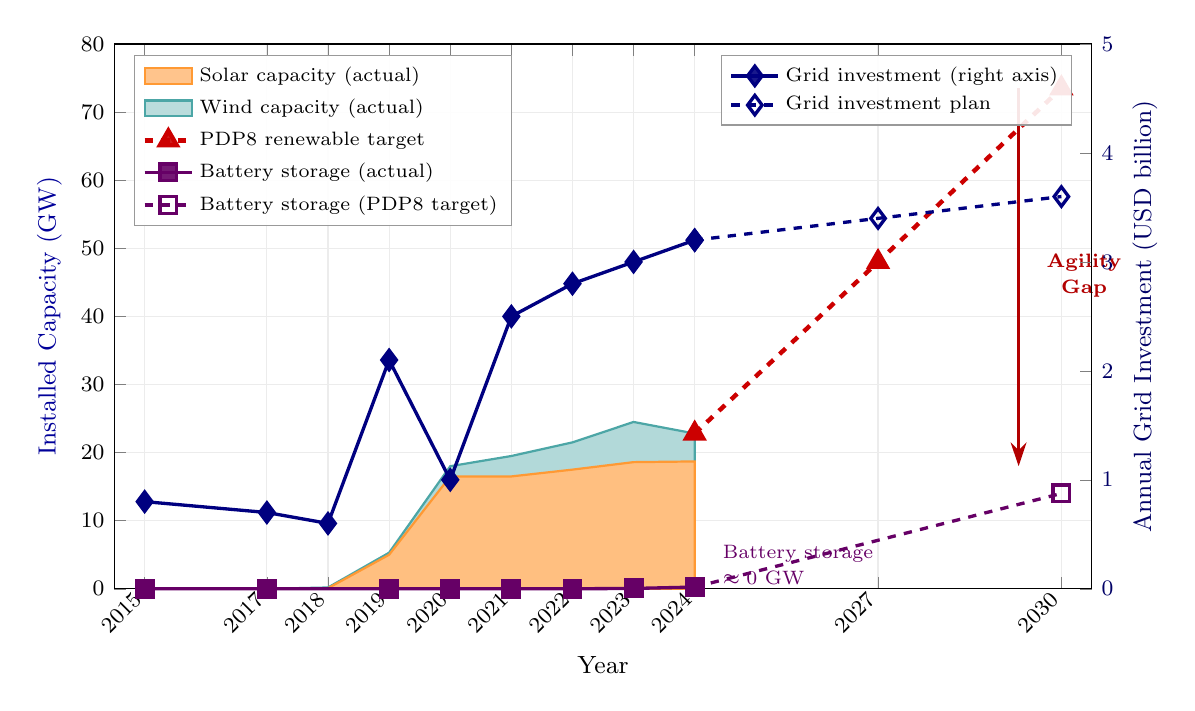
\begin{tikzpicture}
    \pgfplotsset{every x tick label/.append style={/pgf/number format/1000 sep={}}}
    \begin{axis}[
        name=mainaxis,
        width=14cm, height=8.5cm,
        xlabel={Year},
        ylabel={Installed Capacity (GW)},
        axis y line*=left,
        ylabel style={blue!60!black, font=\small},
        xmin=2014.5, xmax=2030.5,
        ymin=0, ymax=80,
        xtick={2015,2017,2018,2019,2020,2021,2022,2023,2024,2027,2030},
        xticklabel style={rotate=45, anchor=east, font=\footnotesize},
        ytick={0,10,20,30,40,50,60,70,80},
        xlabel style={font=\small},
        tick label style={font=\footnotesize},
        legend style={at={(0.02,0.98)}, anchor=north west, font=\scriptsize,
            draw=black!40, fill=white, fill opacity=0.9, text opacity=1,
            cells={anchor=west}, row sep=1pt},
        grid=major,
        grid style={gray!15},
        clip=false,
    ]

    % --- Stacked area: Wind on top of Solar ---
    % Wind layer (total = solar + wind): draw this FIRST so solar overlays
    \addplot[fill=teal!30, draw=teal!70, thick, area legend, forget plot] coordinates {
        (2015, 0.004) (2017, 0) (2018, 0.19) (2019, 5.3) (2020, 18.0)
        (2021, 19.5) (2022, 21.5) (2023, 24.5) (2024, 22.8)
    } \closedcycle;

    % Solar layer (bottom of stack)
    \addplot[fill=orange!50, draw=orange!80, thick, area legend, forget plot] coordinates {
        (2015, 0.004) (2017, 0) (2018, 0.086) (2019, 5.0) (2020, 16.5)
        (2021, 16.5) (2022, 17.5) (2023, 18.6) (2024, 18.7)
    } \closedcycle;

    % Dummy entries for legend (correct order)
    \addlegendimage{area legend, fill=orange!50, draw=orange!80, thick}
    \addlegendentry{Solar capacity (actual)}
    \addlegendimage{area legend, fill=teal!30, draw=teal!70, thick}
    \addlegendentry{Wind capacity (actual)}

    % PDP8 renewable target path (dashed)
    \addplot[red!80!black, ultra thick, dashed, mark=triangle*, mark size=3.5pt,
        mark options={solid, fill=red!80!black}] coordinates {
        (2024, 22.8) (2027, 48.0) (2030, 73.5)
    };
    \addlegendentry{PDP8 renewable target}

    % Battery storage actual (violet, solid)
    \addplot[violet!80!black, very thick, mark=square*, mark size=3pt,
        mark options={solid, fill=violet!80!black}] coordinates {
        (2015, 0) (2017, 0) (2019, 0) (2020, 0) (2021, 0) (2022, 0)
        (2023, 0.05) (2024, 0.25)
    };
    \addlegendentry{Battery storage (actual)}

    % Battery storage PDP8 target (violet, dashed)
    \addplot[violet!80!black, very thick, dashed, mark=square, mark size=3pt,
        mark options={solid, draw=violet!80!black}] coordinates {
        (2024, 0.25) (2030, 14.0)
    };
    \addlegendentry{Battery storage (PDP8 target)}

    % Annotation arrow: agility gap at 2030
    \draw[-{Stealth[length=3mm, width=2mm]}, red!70!black, line width=1.2pt]
        (axis cs:2029.3, 73.5) -- (axis cs:2029.3, 18);
    \node[red!70!black, font=\scriptsize\bfseries, anchor=west] at (axis cs:2029.6, 46)
        {\shortstack{Agility\\Gap}};

    % Annotation: battery near zero
    \node[violet!80!black, font=\scriptsize, anchor=west] at (axis cs:2024.3, 3.5)
        {\shortstack[l]{Battery storage\\$\approx 0$~GW}};

    \end{axis}

    % Right y-axis: Grid investment (overlaid axis)
    \begin{axis}[
        width=14cm, height=8.5cm,
        axis y line*=right,
        axis x line=none,
        xmin=2014.5, xmax=2030.5,
        ymin=0, ymax=5,
        ylabel={Annual Grid Investment (USD billion)},
        ylabel style={blue!40!black, font=\small},
        ytick={0,1,2,3,4,5},
        yticklabel style={font=\footnotesize, blue!40!black},
        legend style={at={(0.98,0.98)}, anchor=north east, font=\scriptsize,
            draw=black!40, fill=white, fill opacity=0.9, text opacity=1,
            cells={anchor=west}},
    ]

    % Grid investment actual
    \addplot[blue!50!black, very thick, mark=diamond*, mark size=3.5pt,
        mark options={solid, fill=blue!50!black}] coordinates {
        (2015, 0.8) (2017, 0.7) (2018, 0.6) (2019, 2.1) (2020, 1.0)
        (2021, 2.5) (2022, 2.8) (2023, 3.0) (2024, 3.2)
    };
    \addlegendentry{Grid investment (right axis)}

    % Grid investment PDP8 plan
    \addplot[blue!50!black, very thick, dashed, mark=diamond, mark size=3.5pt,
        mark options={solid, draw=blue!50!black}] coordinates {
        (2024, 3.2) (2027, 3.4) (2030, 3.6)
    };
    \addlegendentry{Grid investment plan}

    \end{axis}
    \end{tikzpicture}
    \caption{Descriptive evidence for the ``agility gap.'' Left axis: installed renewable capacity (GW), decomposed into solar (orange) and wind (teal). Capacity surged from near-zero in 2017 to 22.8~GW by 2024; PDP8 targets 73.5~GW by 2030. Right axis: annual grid transmission investment (USD billion), which grew modestly from \$0.6--0.8B to \$3.2B. Battery storage (violet) remained near zero through 2024 despite a PDP8 target of 14~GW by 2030. Data: PDP8 (Decision 500/QD-TTg), EVN annual reports, IEA Vietnam Energy Outlook 2023, IRENA.}
    \label{fig:agility_gap_descriptive}
\end{figure}

\section{Literature Review}
There has been a significant amount of environmental policy research utilizing DSGE models to analyze macroeconomic variables.\footnote{See \citet{annicchiarico2015}, \citet{dissou2016}, \citet{annicchiarico2017}, \citet{khan2019}, \citet{chan2020a}, \citet{chan2020b}, \citet{lintunen2021}, and \citet{xiao2022}.}\footnote{Another body of literature that focuses on estimating the Social Cost of Carbon (SCC), called Integrated Assessment Models (IAM). Key works include Nordhaus's DICE/RICE \citep{nordhaus1992, nordhaus1994}, Hope's PAGE \citep{hope2006}, Tol's FUND \citep{tol2002}, and advanced IAMs like WITCH \citep{bosetti2006}, REMIND \citep{bauer2013}, and GCAM \citep{calvin2019}. IAMs face criticism regarding discounting and damage function assumptions \citep{weitzman2009, pindyck2017}. For a review, see \citet{fernandez2025}.} A central debate in E-DSGE research concerns the optimal instrument for emission control under uncertainty. \citet{fischer2011} and \citet{bosetti2013} argue that carbon taxes generally outperform quantity-based instruments (like cap-and-trade) by reducing volatility in critical macroeconomic indicators and effectively lowering emissions. However, other scholars emphasize that these policies cannot be static; \citet{heutel2012} demonstrates that optimal environmental policy must adjust pro-cyclically with the business cycle to mitigate recessionary impacts. More recently, attention has shifted to how these policies interact with structural frictions. For instance, \citet{chan2023} reveals that the complementarity between energy and capital amplifies the transmission of shocks, suggesting that welfare-maximizing carbon taxes must be calibrated lower when endogenous capital utilization is taken into account.

Recently, \citet{airaudo2025green} advanced the Environmental DSGE literature by introducing a New Keynesian small open economy model that captures the macroeconomic costs of the green transition. Their analysis reveals that carbon taxes reduce brown energy use but cause short-term inflation and output losses, a phenomenon they term ``greenflation'', due to limited short-run substitutability between energy and traditional inputs. Crucially, they explicitly model public green investment as a fiscal instrument that can boost the productivity of the green sector. Their findings suggest that while carbon taxes alone are contractionary, mixed strategies that recycle carbon revenues into green public investment yield comparable environmental outcomes at lower welfare costs. 

While \citet{airaudo2025green} focus on the short-run frictional costs of carbon taxation and fiscal policy coordination, this capstone complements their analysis by examining a distinct medium-run friction: the reliability penalty arising from renewable intermittency when flexibility infrastructure lags deployment. Whereas their ``greenflation'' emerges from incomplete factor substitutability under carbon pricing, the present model identifies an additional channel---endogenous grid instability---that operates even absent explicit carbon taxes, driven instead by the physical characteristics of VRE integration. This insight directly informs the policy discussion in Section \ref{sec:conclusion}.

While \citet{airaudo2025green} highlight the short-run frictional costs of transition, a distinct strand of literature rooted in endogenous growth theory offers a mechanism for long-run technological progress through innovation. The Directed Technical Change (DTC) framework, pioneered by \citet{acemoglu2002} and applied to the environment by \citet{acemoglu2012environment}, models innovation as a resource allocation problem where scientists choose which sector to develop. This framework highlights two competing forces: the market size effect, which encourages innovation in the larger sector, and the price effect, which directs innovation toward the sector with higher prices. In the standard model, the market size effect dominates, locking the economy into dirty technologies. However, \citet{acemoglu2012environment} show that policy intervention can manipulate these effects to redirect innovation toward clean technologies.

This theoretical mechanism has found robust empirical support. \citet{popp2002} provided early evidence that higher energy prices significantly induce energy-efficient patenting activity. More recently, \citet{aghion2016} utilized microdata from the global automotive industry to show that firms tend to innovate in areas where they have prior expertise (path dependence), but that fuel price shocks successfully redirect R\&D toward electric and hybrid technologies. Similarly, \citet{calel2016} finds that firms regulated under the EU Emissions Trading System (ETS) increased low-carbon patenting by 10\% compared to a matched control group without crowding out other R\&D, suggesting that policy can effectively steer the direction of technical progress.

However, a fundamental limitation in standard DTC models is the assumption regarding the elasticity of substitution. The AABH framework relies on the premise that clean and dirty inputs are high substitutes. Under this condition, innovation in clean energy allows it to seamlessly replace fossil fuels. Yet, structural analyses challenge this assumption in the presence of intermittency. As renewable penetration rises, the lack of dispatchability renders clean energy an imperfect substitute for baseload fossil generation \citep{hirth2013, joskow2011}. Consequently, models that treat clean capital as a homogeneous block overlook the necessity of complementary innovations. As argued by \citet{hart2019}, when inputs are complements rather than substitutes, technological progress must target not just generation, but the bottleneck technologies---specifically storage---that enable substitutability.

An alternative mechanism for technological progress is learning-by-doing, where costs decline through accumulated production experience rather than explicit R\&D allocation. \citet{arrow1962} first formalized this idea, and it has been widely applied to renewable energy technologies. \citet{nemet2006} documents dramatic cost reductions in solar photovoltaics driven by cumulative deployment, while \citet{kittner2017} shows similar patterns for battery storage. Unlike DTC, learning-by-doing does not require modeling innovation sectors or resource constraints, making it particularly suitable for capturing technological progress in capital goods like batteries where costs decline through manufacturing scale and operational experience.

To address these dynamics, recent contributions have attempted to internalize these physical constraints within general equilibrium frameworks. For instance, \citet{schreiner2020investing} develop a DSGE model for Germany that treats power grid infrastructure as a flexibility option required to bridge the mismatch between variable renewable supply and demand. Crucially, their simulations reveal that while grid investments increase reliability, the associated costs can lead to long-term decreases in GDP and employment unless accompanied by significant efficiency gains. This underscores that solving the intermittency problem is not merely a matter of capital accumulation (building more lines) but requires targeted technological progress in intertemporal substitution (storage).

While the engineering literature has long established the necessity of storage for renewable integration, macroeconomic frameworks have lagged in formally modeling this investment channel. Techno-economic analyses, such as \citet{zakeri2015} and \citet{lund2015}, demonstrate that, as renewable penetration increases, the primary cost driver shifts from generation (LCOE) to flexibility (integration costs). They argue that, without storage, the social cost of intermittency rises nonlinearly due to the need for redundant fossil-fuel backup.

Despite this, the standard E-DSGE literature largely omits storage as an endogenous decision variable. Major recent contributions, including \citet{batten2020} and \citet{annicchiarico2021}, focus predominantly on pricing instruments (carbon taxes) or quantity restrictions (caps), effectively assuming that energy markets clear instantaneously. When backup is modeled, as in \citet{schreiner2020investing}, it is often treated as a static infrastructure cost or fossil generation, which inherently reintroduces carbon emissions or capital rigidities that dampen the efficacy of green transition policies.

This creates a significant modeling gap. By treating backup as fossil generation rather than intertemporal substitution, existing models fail to capture the capital-intensive nature of grid stability. As noted by \citet{kittner2017}, the declining costs of battery technologies imply that energy storage is transitioning from a niche ancillary service to a core infrastructure asset. Consequently, accurately capturing the ``greenflation'' trade-off requires a framework where agents can optimize investment not just in productive capital, but also in smoothing capital (BESS), a structural feature this capstone seeks to integrate.

Beyond the storage modeling gap, international trade emerges as a critical transmission channel for small open economies navigating the green transition. Open-economy macroeconomic research shows that energy price shocks behave like terms-of-trade shocks and can generate persistent effects on output, inflation, and external balances when a country is heavily dependent on imported energy \citep{obstfeld1995, corsetti2010}. In the environmental domain, a growing body of open-economy E-DSGE and two-country DSGE studies demonstrates that integrating carbon pricing across borders induces spillovers in trade flows, alters the competitiveness of carbon-intensive sectors, and raises carbon leakage risks \citep{bohringer2018, balke2022}. These mechanisms matter quantitatively: recent guidance by the Network for Greening the Financial System \citep{ngfs2022} and the IMF \citep{imf2021} emphasizes that external exposure, particularly dependence on imported energy and intermediate goods, amplifies transition-related price shocks and materially affects domestic inflation and output under decarbonization scenarios.

For Vietnam specifically, trade linkages are not peripheral but central to its green-transition challenge. The country's rapid export-oriented industrialization has been accompanied by rising dependence on imported thermal coal and liquefied natural gas (LNG), making global fossil-fuel price fluctuations a direct source of domestic production-cost volatility \citep{iea2023, gso2024}. At the same time, Vietnam's energy-intensive export sectors, such as steel, cement, and fertilizers, face increasing exposure to foreign climate policies like the EU Carbon Border Adjustment Mechanism \citep{ec2023}. Empirical work on Vietnam and comparable emerging economies shows that trade openness interacts strongly with renewable-energy adoption and CO\textsubscript{2} emissions, reinforcing the need to jointly consider trade and environmental policy in macro-modeling \citep{almulali2015, vo2020}. The broader literature on carbon leakage, border adjustments, and greenflation also underscores the relevance of modelling international connections: unilateral carbon pricing, carbon-border tariffs, or linked carbon markets produce measurable welfare, competitiveness, and terms-of-trade effects that an open-economy E-DSGE is well-suited to analyze \citep{fischer2012, bohringer2022}. These insights collectively highlight that, for a highly open economy like Vietnam, international trade in both energy and goods is not an auxiliary consideration but a defining structural feature of the green transition.

Taken together, the existing literature provides a strong foundation for environmental DSGE frameworks, yet it leaves critical blind spots regarding the interactions among intermittency, flexibility investment, and induced innovation. Building on these gaps, this capstone makes three core contributions. First, it introduces an endogenous reliability function that links capital utilization to the ratio of flexibility assets to renewable volatility, allowing intermittency to propagate through both the production function and the investment channel. Second, it incorporates reliability-gap-induced learning-by-doing in Battery Energy Storage Systems (BESS), where technological progress responds endogenously to the gap between target and actual grid reliability, a channel distinct from frontier R\&D allocation. Third, it distinguishes between agile private battery investment and slow-moving public grid infrastructure, capturing the structural \textit{agility gap} observed in developing economies. By integrating these elements, the capstone argues that market-based signals are essential complements to storage investment in transforming the green transition from a cost burden into a sustainable growth path.

\section{Methodology} \label{sec:methodology}

\subsection{Model Overview}

I develop a Small Open Economy Dynamic Stochastic General Equilibrium (DSGE) model calibrated to Vietnam. The model is designed to analyze the macroeconomic consequences of renewable-energy intermittency when the accumulation of grid flexibility lags behind the expansion of variable renewable generation, while capturing the external balance implications through international borrowing and lending. The framework extends standard Environmental DSGE (E-DSGE) models by introducing two departures from the canonical structure.

First, grid reliability is endogenized as a technological constraint on effective capital services rather than treated implicitly through energy prices or exogenous productivity shocks. This reflects the physical reality that electricity systems with high renewable penetration are constrained by temporal mismatches between supply and demand. Second, I embed a price-induced learning-by-doing mechanism that governs the rate of cost reduction in battery storage technologies. This allows the economy to respond endogenously to reliability scarcity through technological progress rather than relying solely on capital accumulation or policy intervention.

The economy consists of a representative household and a representative firm operating in a small open economy with access to international bond markets. Households supply labor, accumulate productive capital, and trade bonds with the rest of the world at a debt-elastic interest rate. Firms produce final output using a CES aggregator of value-added (from capital and labor) and a fixed energy endowment. Grid reliability is determined endogenously by the stock of flexibility assets (batteries and grid infrastructure) relative to renewable volatility. Battery costs decline through reliability-gap-induced learning-by-doing, while public grid investment follows a rule-based response to reliability shortfalls.

A central modeling choice is the treatment of capital utilization. In contrast to standard RBC or New Keynesian models, capital utilization in this framework is not a choice variable and does not affect depreciation. Instead, it reflects the fraction of installed productive capital that is operational given the state of grid reliability. This interpretation aligns utilization with system-wide power availability rather than firm-level intensity of use.

\subsection{Households} \label{sec:households}

A representative household maximizes expected lifetime utility:
\begin{equation}
\mathbb{E}_0 \sum_{t=0}^{\infty} \beta^t
\left[
\log(C_t) - \frac{L_t^{1+\sigma_L}}{1+\sigma_L}
\right]
\end{equation}

subject to the budget constraint:
\begin{equation}
C_t + I_{p,t} + P_{bat,t} I_{bat,t} + B^*_t + T_t
=
Y_t + (1+r^*_{t-1}) B^*_{t-1}
\label{eq:hh_budget}
\end{equation}

where $I_{p,t}$ is productive capital investment, $I_{bat,t}$ battery investment at world price $P_{bat,t}$, $B^*_t$ denotes net foreign asset holdings earning the country-specific interest rate $r^*_t$, and $T_t$ is a lump-sum tax levied by the government to finance public grid investment (specified in Section~\ref{sec:government}).

The household chooses $\{C_t, L_t, K_{p,t+1}, B^*_t\}$ to maximize utility subject to the budget constraint. The first-order conditions are derived as follows.

\paragraph{Euler equation for capital.} Differentiating the Lagrangian with respect to $K_{p,t+1}$ and $C_t$, and noting that the marginal product of capital in the production function is $\partial Y_{t+1} / \partial K_{p,t} = \alpha Y_{t+1}/K_{p,t}$ (from the Cobb-Douglas value-added structure in equation~\ref{eq:value_added} below), the intertemporal optimality condition equates the marginal cost of investing one unit of consumption today with the discounted marginal benefit of the return tomorrow:
\begin{equation}
\frac{1}{C_t} = \beta \mathbb{E}_t \left[ \frac{\alpha Y_{t+1}/K_{p,t+1} + 1 - \delta_p}{C_{t+1}} \right]
\label{eq:euler}
\end{equation}

\noindent \textit{In words:} the household invests in capital until the cost of forgoing one unit of consumption today ($1/C_t$) equals the expected discounted benefit of the gross return---marginal product plus undepreciated capital---valued at tomorrow's marginal utility ($1/C_{t+1}$).

\paragraph{Labor supply.} Differentiating with respect to $L_t$ and equating the marginal disutility of labor ($L_t^{\sigma_L}$) with the marginal utility of the real wage ($w_t/C_t$), and substituting the competitive wage $w_t = (1-\alpha)V_t/L_t$ from the firm's profit maximization:
\begin{equation}
(1-\alpha) V_t = \varphi \, C_t \, L_t^{1+\sigma_L}
\label{eq:labor_supply}
\end{equation}

\noindent \textit{In words:} the labor share of value-added (left side) equals the household's required compensation for working, which is increasing in consumption (higher income households demand more leisure) and steeply increasing in hours worked (via the exponent $1+\sigma_L$). The parameter $\varphi$ is the labor disutility weight, calibrated endogenously to match steady-state labor hours of $L_{ss} = 0.33$.

\subsection{The Production Sector}

\subsubsection{Final Goods Production}

Final output $Y_t$ is produced by a representative firm using a nested Constant Elasticity of Substitution (CES) technology that combines value-added and energy inputs. To reduce notational clutter in the CES expressions that follow, I adopt the convention of writing exponents in terms of the \textit{substitution parameter} $s \equiv (\sigma - 1)/\sigma$ for a given elasticity $\sigma$. When $\sigma < 1$ (complements), $s < 0$; when $\sigma > 1$ (substitutes), $s > 0$; when $\sigma = 1$ (Cobb-Douglas), $s = 0$. Using $s_E \equiv (\sigma_E - 1)/\sigma_E$ for the output aggregator:

\begin{equation}
Y_t = \left[(1-\omega_E)V_t^{s_E} + \omega_E \bar{E}^{s_E}\right]^{1/s_E}
\label{eq:final_output}
\end{equation}

\noindent \textit{In words:} output is a weighted aggregate of value-added $V_t$ and energy $E_t$, where neither input can fully substitute for the other when $\sigma_E < 1$. Shutting down either input drives output toward zero---energy and productive activity are essential complements.

This formulation follows the environmental macroeconomics literature \citep{heutel2012, airaudo2025green} and captures the limited short-run substitutability between energy and non-energy inputs. When the elasticity of substitution $\sigma_E$ is low (calibrated at 0.6), disruptions to energy supply translate into disproportionately large output losses, a feature that is empirically relevant for energy-intensive emerging economies.

Value-added production combines labor and effective capital services:

\begin{equation}
V_t = (u_t K_{p,t})^\alpha L_t^{1-\alpha}
\label{eq:value_added}
\end{equation}

\noindent \textit{In words:} value-added is produced from ``effective capital'' $u_t K_{p,t}$---the fraction of installed capacity that is actually operational---combined with labor. A factory with machines that cannot run due to power outages produces less, even if the machines physically exist.

Here, $K_{p,t}$ is the physical stock of productive capital, and $u_t \in (0,1)$ represents the fraction of capital that can be operated given grid conditions. Unlike standard utilization models (e.g., \citet{greenwood1988}), $u_t$ is not chosen optimally by firms and does not influence capital depreciation. Instead, it captures system-wide outages, curtailment, and power shortages that prevent installed capital from being used. In this sense, grid instability manifests as an endogenous, state-dependent productivity wedge: a 3\% reliability shortfall ($u_t = 0.97$) is equivalent to a TFP loss of approximately $\alpha \times 3\% \approx 1\%$.

In the implemented model, energy enters the CES aggregator as a fixed endowment $\bar{E}$, reflecting the assumption that total energy supply is determined by installed capacity and policy targets (PDP8) rather than optimized period-by-period. This simplification allows the model to focus on the key channel of interest---how renewable intermittency affects grid reliability and, through it, effective capital utilization---without requiring a full energy market clearing block. The intermittency shock enters through the reliability function (equation \eqref{eq:utilization} below) rather than through energy supply directly.

The household's optimality conditions---the capital Euler equation \eqref{eq:euler} and labor supply condition \eqref{eq:labor_supply}, as derived in Section~\ref{sec:households}---together with the production technology determine the equilibrium allocation of capital and labor.

\subsection{Grid Reliability and Flexibility Assets}

\subsubsection{Reliability Constraint}

Grid reliability is modeled as a reduced-form approximation to the probability that aggregate electricity demand can be met without load shedding. The functional form is motivated by the standard reliability engineering framework, where the Loss-of-Load Probability (LOLP) declines exponentially as reserve margins (here, flexibility assets) increase relative to demand uncertainty (here, renewable volatility). In engineering practice, LOLP is defined as the probability that available generation falls short of demand in a given period; the complement $1 - \text{LOLP}$ measures the fraction of time the system operates reliably. The exponential form $u = 1 - \exp(-z)$ is the simplest functional form that maps a non-negative ``adequacy ratio'' $z \geq 0$ into a probability bounded on $(0,1)$, while preserving the key engineering property that additional reserves exhibit diminishing marginal returns to reliability. This is the same mathematical structure underlying the Poisson reliability model widely used in power systems analysis \citep{zakeri2015, lund2015}.

The reliability constraint is formalized as:

\begin{equation}
u_t = 1 - \exp\left(-\psi \frac{F_t}{\phi_{int} \cdot \text{Vol}_{ren,t}}\right)
\label{eq:utilization}
\end{equation}

\noindent \textit{In words:} grid reliability is an increasing, concave function of the ratio of flexibility assets ($F_t$) to renewable volatility ($\text{Vol}_{ren,t}$). When the system has abundant flexibility relative to volatility, nearly all capital can operate ($u_t \approx 1$). When flexibility is scarce, outages proliferate and utilization collapses.

The variables and parameters are:
\begin{itemize}
    \item $F_t$ is the stock of flexibility assets (batteries + grid infrastructure, defined below)
    \item $\phi_{int} > 0$ is a scaling parameter that converts renewable volatility into effective flexibility requirements; it captures the complexity of integrating variable renewables into the grid (calibrated endogenously to $\approx 55.6$)
    \item $\text{Vol}_{ren,t}$ measures renewable output volatility (strictly positive)
    \item $\psi > 0$ governs the sensitivity of reliability to the flexibility-to-volatility ratio (calibrated at 2.0)
\end{itemize}

This exponential formulation ensures that:
\begin{enumerate}
    \item When $F_t \to \infty$, utilization approaches unity (perfect reliability): $u_t \to 1$
    \item When $F_t \to 0$, utilization approaches zero (grid collapse): $u_t \to 0$
    \item The function is always bounded: $u_t \in (0, 1)$ for all $F_t > 0$
    \item Marginal returns to flexibility are strictly diminishing
    \item The reliability penalty increases exponentially with the volatility-to-flexibility ratio
\end{enumerate}

This exponential functional form is standard in reliability engineering \citep{zakeri2015, lund2015} and ensures that flexibility requirements rise nonlinearly as VRE penetration increases, capturing the convex integration costs documented in the empirical literature.

To illustrate the nonlinearity, Table~\ref{tab:reliability_numerical} reports the reliability response to flexibility shortfalls under the baseline calibration. The convex curvature is evident: a 10\% flexibility deficit reduces reliability by 1.26 percentage points (pp), but a 50\% deficit causes a 14.32~pp collapse---more than 11 times the proportional response. This accelerating penalty captures the engineering reality that the first units of flexibility (spinning reserves, fast-ramping gas) are cheap and effective, while maintaining reliability under extreme shortfalls requires exponentially more resources.

\begin{table}[H]
    \centering
    \caption{\textbf{Reliability Response to Flexibility Shortfalls}}
    \label{tab:reliability_numerical}
    \renewcommand{\arraystretch}{1.3}
    \small
    \begin{tabular}{c c c c}
        \toprule
        \textbf{Flexibility Shortfall} & \textbf{Reliability ($u_t$)} & \textbf{Reliability Loss (pp)} & \textbf{Approx. Output Loss} \\
        \midrule
        0\% (steady state) & 97.00\% & --- & --- \\
        $-5$\% & 96.43\% & 0.57 & $-0.21$\% \\
        $-10$\% & 95.74\% & 1.26 & $-0.45$\% \\
        $-20$\% & 93.95\% & 3.05 & $-1.10$\% \\
        $-30$\% & 91.41\% & 5.59 & $-2.02$\% \\
        $-50$\% & 82.68\% & 14.32 & $-5.17$\% \\
        \bottomrule
    \end{tabular}
    \vspace{0.2cm}
    \parbox{\textwidth}{\footnotesize \textit{Note:} Computed from equation~\eqref{eq:utilization} under the baseline calibration ($\psi = 2.0$, $\phi_{int} = 55.6$). Output loss approximated as $\alpha \times \Delta u / u_{ss}$, capturing the direct effective-capital channel. The convexity of the reliability function implies that moderate flexibility shortfalls (10--20\%) have manageable consequences, but large deficits trigger disproportionate reliability collapses---motivating the ``Reliability Valley'' analysis in Section~\ref{sec:results}.}
\end{table}

The volatility term captures the absolute variability of renewable generation:
\begin{equation}
\overline{\text{Vol}}_{ren} = \theta_{ren} \cdot K_{ren} \cdot \sigma_{ren}
\label{eq:renewable_volatility}
\end{equation}

where $\theta_{ren}$ is the renewable penetration share, $K_{ren}$ is installed renewable capacity, and $\sigma_{ren}$ is the standard deviation of the intermittency shock. In the quantitative implementation, $\overline{\text{Vol}}_{ren}$ is treated as a \textbf{calibrated parameter} (not an endogenous variable), set to match the baseline renewable fleet characteristics under PDP8. This model deliberately treats the trajectory of Variable Renewable Energy (VRE) deployment as exogenous. The firms do not dynamically optimize how many solar panels to build based on current prices; instead, VRE capacity follows the government's PDP8 plan implicitly. This simplification isolates the endogenous response of flexibility assets (the ``agility gap''). Future models could endogenize VRE investment explicitly. The intermittency shock $\varepsilon_{ren,t}$ enters the reliability function~\eqref{eq:utilization} multiplicatively as $\overline{\text{Vol}}_{ren} \cdot \exp(\varepsilon_{ren,t})$, generating stochastic variation in effective volatility around the calibrated baseline.

Conceptually, $\overline{\text{Vol}}_{ren}$ varies with the size of the renewable fleet, capturing the empirical finding that integration costs rise with penetration \citep{hirth2013}. In the deterministic transition simulations (Section~\ref{subsec:valley}), $\overline{\text{Vol}}_{ren}$ is allowed to increase along the policy-determined VRE expansion path.

\subsubsection{Public and Private Flexibility Assets}

Total system flexibility $F_t$ is produced by combining two distinct assets: private battery storage and public grid infrastructure. These assets serve complementary roles. Battery storage shifts energy \textit{across time} (charging when supply exceeds demand, discharging when it falls short), while grid infrastructure shifts energy \textit{across space} (transmitting power from surplus to deficit regions). Using the shorthand $s_F \equiv (\rho - 1)/\rho$ for the flexibility substitution parameter (where $\rho$ is the elasticity of substitution between battery and grid capital), the flexibility bundle is:

\begin{equation}
F_t =
\left[
\mu (A_{bat,t} K_{b,t})^{s_F}
+
(1-\mu) K_{g,t}^{s_F}
\right]^{1/s_F},
\qquad \rho < 1 \;\Leftrightarrow\; s_F < 0
\label{eq:flexibility_bundle}
\end{equation}

\noindent \textit{In words:} flexibility is a weighted combination of technology-augmented battery capacity ($A_{bat,t} K_{b,t}$) and grid infrastructure ($K_{g,t}$), where neither can fully replace the other. A grid with abundant batteries but no transmission lines cannot deliver stored power; a grid with extensive transmission but no storage cannot smooth intermittent supply. The negative exponent $s_F < 0$ (since $\rho = 0.4 < 1$) ensures that flexibility collapses if either input approaches zero---a mathematical expression of the engineering constraint.

The elasticity of substitution $\rho = 0.4$ is calibrated below unity to enforce this complementarity. The parameter $\mu = 0.16$ governs the relative weight of battery storage in the aggregate, reflecting Vietnam's current early-stage storage deployment. Innovation affects flexibility through $A_{bat,t}$, which represents learning-by-doing that reduces the effective cost of battery storage services. Improvements in storage technology raise the usable energy-shifting capacity per unit of installed storage rather than merely increasing physical capacity.

The complementarity parameter $\rho < 1$ has a precise formal consequence for the returns to coordinated flexibility investment.

\begin{proposition}[Superadditivity of Joint Flexibility Investment] \label{prop:superadditivity}
Let $F(x, y) = [\mu \, x^{s} + (1-\mu) \, y^{s}]^{1/s}$ be the CES flexibility aggregator with $s \equiv (\rho - 1)/\rho$, $\mu \in (0,1)$, and $\rho \in (0,1)$ (so that $s < 0$). For any baseline inputs $x_0, y_0 > 0$ and scaling factor $\lambda > 1$, the joint gain from scaling both inputs strictly exceeds the sum of individual gains:
\begin{equation*}
\underbrace{F(\lambda x_0, \lambda y_0) - F(x_0, y_0)}_{\textit{joint gain}} \;>\; \underbrace{\bigl[F(\lambda x_0, y_0) - F(x_0, y_0)\bigr]}_{\textit{battery-only gain}} + \underbrace{\bigl[F(x_0, \lambda y_0) - F(x_0, y_0)\bigr]}_{\textit{grid-only gain}}
\end{equation*}
\end{proposition}

\noindent The result follows from the strict supermodularity of the CES aggregator when inputs are complements ($\rho < 1$). The formal proof is provided in Appendix~\ref{app:proof_superadditivity}.\footnote{The proposition is a direct consequence of the CES functional form with $\rho < 1$, which implies complementarity between battery storage and grid capital. The restriction $\rho < 1$ (i.e., $s < 0$) ensures a strictly positive cross-partial $\partial^2 F / \partial x \, \partial y > 0$, from which superadditivity follows via Topkis's theorem \citep{topkis1998}.}

\noindent \textbf{Remark.} By homogeneity of degree one, the joint gain equals exactly $(\lambda - 1) F(x_0, y_0)$. Each individual gain is strictly less than $(\lambda-1) F$ due to the strict concavity of $F$ in each argument separately. The \textit{superadditivity gap}---the excess of the joint gain over the sum of individual gains---measures the pure complementarity premium from coordinated investment. This gap vanishes only as $\rho \to 1$ (perfect substitutes) and grows as $\rho \to 0$ (Leontief). Table~\ref{tab:ces_complementarity} evaluates the gap numerically under the baseline calibration.

\begin{table}[H]
    \centering
    \caption{\textbf{CES Flexibility: Superadditivity Under Baseline Calibration}}
    \label{tab:ces_complementarity}
    \renewcommand{\arraystretch}{1.3}
    \small
    \begin{tabular}{l c c}
        \toprule
        \textbf{Scenario} & \textbf{Flexibility ($F$)} & \textbf{Change from Baseline} \\
        \midrule
        Baseline ($K_b = 0.19$, $K_g = 1.14$) & 0.526 & --- \\
        Double $K_b$ only ($K_b = 0.38$) & 0.809 & $+53.9$\% \\
        Double $K_g$ only ($K_g = 2.28$) & 0.596 & $+13.2$\% \\
        Double both & 1.052 & $+100.0$\% \\
        \midrule
        Sum of individual gains & --- & $+67.1$\% \\
        Joint gain (Proposition~\ref{prop:superadditivity}) & --- & $+100.0$\% \\
        Superadditivity gap & --- & $+32.9$ pp \\
        \bottomrule
    \end{tabular}
    \vspace{0.2cm}
    \parbox{\textwidth}{\footnotesize \textit{Note:} Computed from equation~\eqref{eq:flexibility_bundle} with $\rho = 0.4$, $\mu = 0.16$, $A_{bat} = 1$, $\lambda = 2$. The 32.9 percentage point superadditivity gap quantifies the complementarity premium. By Proposition~\ref{prop:superadditivity}, this gap is strictly positive for any $\rho < 1$. Battery capital has a larger individual marginal effect because $\mu = 0.16$ places it in the scarce-factor position within the CES aggregator.}
\end{table}

\subsubsection{Laws of Motion}

Public grid capital evolves according to a standard accumulation equation:

\begin{equation}
K_{g,t+1} = (1-\delta_g)K_{g,t} + I_{grid,t}
\label{eq:grid_capital}
\end{equation}

Grid investment is undertaken by the government and is subject to institutional inertia, reflecting planning delays and construction lags. As a result, public flexibility adjusts slowly to changes in renewable penetration.

Private battery capital evolves as:

\begin{equation}
K_{b,t+1} = (1-\delta_b)K_{b,t} + I_{bat,t}
\label{eq:battery_capital}
\end{equation}

Battery capital follows a standard linear accumulation law without adjustment costs, as the modular and scalable nature of battery storage allows rapid deployment without the installation frictions typically associated with heavy infrastructure.

\paragraph{Battery Investment Decision.}
To motivate the battery investment rule, I derive the shadow rental rate on storage services from the model's first-order conditions. The marginal value of an additional unit of battery capital flows through the chain $K_b \to F \to u \to V \to Y$:

\begin{equation}
R_{b,t} \;\equiv\; \frac{\partial Y_t}{\partial F_t} \cdot \frac{\partial F_t}{\partial (A_{bat,t} K_{b,t-1})} \cdot A_{bat,t}
\label{eq:rental_rate}
\end{equation}

Each component is computed from the model's structural equations. From the CES flexibility aggregator \eqref{eq:flexibility_bundle}:
\begin{equation}
\frac{\partial F_t}{\partial (A_{bat,t} K_{b,t-1})} = \mu \left(\frac{A_{bat,t} K_{b,t-1}}{F_t}\right)^{-1/\rho_f}
\label{eq:dF_dKb}
\end{equation}

The marginal product of flexibility in output operates through the reliability channel. Combining the exponential reliability function \eqref{eq:utilization} with the value-added function \eqref{eq:value_added} and the CES output aggregator \eqref{eq:final_output}:
\begin{equation}
\frac{\partial Y_t}{\partial F_t} = \underbrace{\frac{\partial Y_t}{\partial V_t}}_{\text{CES share}} \cdot \underbrace{\frac{\partial V_t}{\partial u_t}}_{\text{capital utilization}} \cdot \underbrace{\frac{\partial u_t}{\partial F_t}}_{\text{reliability gradient}} = \frac{\partial Y_t}{\partial V_t} \cdot \alpha \frac{V_t}{u_t} \cdot \frac{\psi (1 - u_t)}{\phi_{int} \cdot \text{Vol}_{ren,t}}
\label{eq:dY_dF}
\end{equation}

where $\partial u_t / \partial F_t = \psi(1-u_t)/(\phi_{int} \cdot \text{Vol}_{ren,t})$ follows from differentiating the exponential reliability function, and $\partial V_t / \partial u_t = \alpha V_t / u_t$ from the Cobb-Douglas value-added specification. Note that $R_{b,t}$ is increasing in the reliability gap $(1-u_t)$: when reliability falls below target, the marginal return to storage rises sharply due to the exponential curvature of the reliability function.

Table~\ref{tab:mpk_decomp} evaluates each component of the chain at steady-state values, yielding a shadow rental rate of $R_{b,ss} = 10.93\%$ quarterly. The decomposition reveals that the \textit{flexibility bottleneck}---the large marginal product of batteries in the CES aggregator ($\partial F / \partial(A_{bat} K_b) = 2.04$)---is the dominant force, reflecting the scarcity of storage relative to grid capital. The reliability gradient ($\partial u / \partial F = 0.20$) is moderate because the system operates near the flat portion of the exponential curve at $u_{ss} = 0.97$.

\begin{table}[H]
    \centering
    \caption{\textbf{Marginal Product Decomposition of Battery Rental Rate ($R_{b,ss}$)}}
    \label{tab:mpk_decomp}
    \renewcommand{\arraystretch}{1.3}
    \small
    \begin{tabular}{l l c l}
        \toprule
        \textbf{Component} & \textbf{Expression} & \textbf{Value} & \textbf{Interpretation} \\
        \midrule
        CES output share & $\partial Y / \partial V$ & 0.725 & Value-added dominates output \\
        Utilization effect & $\partial V / \partial u = \alpha V/u$ & 0.370 & Capital utilization channel \\
        Reliability gradient & $\partial u / \partial F$ & 0.200 & Moderate (near flat of exp.\ curve) \\
        Flexibility bottleneck & $\partial F / \partial (A_{bat} K_b)$ & 2.040 & Scarce factor in CES \\
        \midrule
        \textbf{Shadow rental rate} & $R_{b,ss}$ & \textbf{0.109} & \textbf{10.93\% quarterly} \\
        \bottomrule
    \end{tabular}
    \vspace{0.2cm}
    \parbox{\textwidth}{\footnotesize \textit{Note:} Evaluated at the deterministic steady state. $R_{b,ss} = (\partial Y/\partial V) \times (\partial V/\partial u) \times (\partial u/\partial F) \times (\partial F/\partial(A_{bat} K_b)) \times A_{bat} = 0.725 \times 0.370 \times 0.200 \times 2.040 \times 1.0 = 0.109$. The large flexibility bottleneck term reflects batteries' position as the scarce factor ($\mu = 0.16$) in the CES aggregator. When $u_t$ falls below target, the reliability gradient steepens (since $\partial u/\partial F \propto (1-u_t)$), amplifying $R_b$ and triggering the investment response.}
\end{table}

In the computational implementation, the investment rule takes the reduced form:
\begin{equation}
\frac{I_{bat,t}}{\bar{I}_{bat}} = \left(\frac{u^*}{u_t}\right)^{\phi_{grid}} \cdot \frac{1}{P_{bat,t}}
\label{eq:battery_investment}
\end{equation}

\noindent \textit{In words:} battery investment rises above its steady-state level when reliability falls below target, and falls when batteries become more expensive.

\textbf{Modeling Choice Justification:} A fully endogenous, forward-looking optimization of battery capital by firms---subject to the highly non-linear exponential reliability constraint---would create massive non-convexities and complicate the Blanchard-Kahn conditions required for local approximation. The reduced-form rule in Equation~\eqref{eq:battery_investment} mathematically proxies the gradient of the shadow price while keeping the system computationally tractable and ensuring local saddle-path stability.

The connection between this reduced form and the structural FOC chain (equations~\ref{eq:rental_rate}--\ref{eq:dY_dF}) operates as follows. The rental rate $R_{b,t}$ depends on the reliability gradient $\partial u / \partial F = \psi(1-u_t)/(\phi_{int} \cdot \text{Vol}_{ren,t})$, which is proportional to the reliability gap $(1-u_t)$. When reliability falls below target, $(1-u_t)$ rises, steepening the gradient and raising $R_{b,t}$ above its steady-state value. The ratio $u^*/u_t$ is a monotone transformation of this gap: at steady state $u_t = u^* = 0.97$ and the ratio equals unity; when $u_t$ drops below $u^*$, the ratio rises, driving investment above replacement levels. The exponent $\phi_{grid}$ governs the elasticity of the investment response to the reliability gap---higher values imply more aggressive battery deployment when the grid is stressed. The price term $1/P_{bat,t}$ reflects the cost side: Vietnam is a price-taker in global battery markets, so higher world battery prices reduce real investment even when the return to storage is high. At steady state, the rule collapses to $I_{bat,ss}/\bar{I}_{bat} = 1$, consistent with capital replacement at $I_{bat,ss} = \delta_b K_{b,ss}$.

\subsection{Learning-by-Doing in Battery Technology}

Technological progress in battery storage reflects cumulative deployment experience rather than explicit R\&D allocation. The evolution of battery technology follows:
\begin{equation}
A_{bat,t} = \underbrace{A_{bat,t-1}}_{\text{inherited knowledge}} \times \left(1 + \underbrace{\eta_{bat}}_{\text{learning rate}} \cdot \underbrace{\chi}_{\substack{\text{signal}\\\text{transmission}}} \cdot \underbrace{\frac{u^* - u_t}{u^*}}_{\text{reliability gap}}\right)
\label{eq:learning_by_doing}
\end{equation}

where:
\begin{itemize}
    \item $\eta_{bat} > 0$ is the learning-by-doing elasticity
    \item $\chi \in (0,1]$ captures regulatory distortions in price signals
    \item $u^*$ is the target reliability level
    \item $u_t$ is the current reliability
\end{itemize}

This specification ensures that technological progress is zero when reliability is at target ($u_t = u^*$) and accelerates proportionally when reliability falls below target. The growth rate is bounded and mean-reverting, consistent with empirical learning curves that exhibit saturation effects \citep{nemet2006}. The reliability gap $(u^* - u_t)/u^*$ serves as the scarcity signal: when the grid is stressed, the economic value of improved storage technology rises, inducing faster learning.

The parameter $\chi$ captures regulatory distortions that dampen the transmission of reliability scarcity into private incentives. In regulated markets with incomplete remuneration for ancillary services (e.g., fixed tariffs, lack of capacity payments, or missing real-time pricing), $\chi < 1$, weakening learning responses even when flexibility is scarce. In fully liberalized markets with scarcity pricing, $\chi = 1$.

\textbf{Policy Implication for Vietnam:} In the specific context of Vietnam, the state utility (EVN) currently operates with strictly regulated retail tariffs and lacks a mature Competitive Wholesale or Retail Electricity Market (VWEM/VREM) tailored for dynamic capacity pricing. Therefore, Vietnam's current regulatory baseline corresponds to a $\chi$ significantly below 1 (close to 0). This formalizes a critical policy recommendation: to unlock the learning-by-doing channel for battery storage, Vietnam must accelerate its transition toward competitive markets featuring time-of-use (ToU) and capacity payments. Without these scarcity signals, technological progress will stagnate regardless of the physical need for flexibility.

This formulation differs from Directed Technical Change in three key respects. First, there is no R\&D sector or explicit allocation of scientists. Second, technological progress responds to the \textit{reliability gap} rather than inter-sectoral competition. Third, learning is embodied in deployment rather than disembodied knowledge creation.

\subsection{Reliability as the Scarcity Signal}

In this model, the reliability gap $(u^* - u_t)/u^*$ serves as the endogenous scarcity signal that drives both investment and learning responses. This formulation has a natural economic interpretation: the marginal benefit of additional flexibility is proportional to the current reliability shortfall $(1-u_t)$, a property inherited from the exponential specification of the utilization function.

From the utilization function \eqref{eq:utilization}, the marginal effect of flexibility on reliability is:
\begin{equation}
\frac{\partial u_t}{\partial F_t} = (1 - u_t) \cdot \frac{\psi}{\phi_{int} \cdot \text{Vol}_{ren,t}}
\end{equation}

When reliability is already high (near unity), additional flexibility yields diminishing returns. When reliability is low (large shortfall), flexibility becomes critically valuable. Both the battery investment rule \eqref{eq:battery_investment} and the learning-by-doing equation \eqref{eq:learning_by_doing} respond to this scarcity through the ratio $u^*/u_t$, which rises when reliability falls below target.


\subsection{Government} \label{sec:government}

The government does not solve a Ramsey optimization problem. Instead, it follows an institutional reliability-targeting rule motivated by Vietnam's Power Development Plan 8 (PDP8). Public grid investment responds mechanically to deviations of reliability from a target level:

\begin{equation}
\frac{I_{grid,t}}{\bar{I}_{grid}} =
\left(\frac{u^*}{u_t}\right)^{\phi_{grid}}
\exp(\varepsilon_{I,t})
\label{eq:grid_investment_rule}
\end{equation}

\noindent \textit{In words:} the government spends more on grid infrastructure when reliability falls below target, and less when the grid is performing well. This rule is structurally identical to the battery investment rule \eqref{eq:battery_investment} except that it lacks a price term (grid investment uses domestically produced goods) and includes an implementation shock $\varepsilon_{I,t}$ reflecting bureaucratic delays, procurement bottlenecks, and construction lags.

This rule captures the reactive nature of infrastructure policy, where investment accelerates following reliability crises rather than anticipating them. The parameter $\phi_{grid}$ governs the aggressiveness of the fiscal response.

The government runs a balanced budget each period, financing grid investment through lump-sum taxes $T_t$ levied on the representative household:
\begin{equation}
T_t = I_{grid,t}
\label{eq:gov_budget}
\end{equation}

The government does not optimize; it follows the mechanical investment rule above and balances its budget period-by-period through lump-sum taxation.

\subsection{Battery Price Dynamics}

Battery investment goods are priced at world price $P_{bat,t}$, which enters the resource constraint and the battery investment rule. The world price of batteries evolves according to a persistent AR(1) process:
\begin{equation}
\log P_{bat,t} = \rho_{bat} \log P_{bat,t-1} + \varepsilon_{bat,t}
\label{eq:battery_price_shock}
\end{equation}

where $\varepsilon_{bat,t} \sim N(0, \sigma^2_{bat})$ captures global shocks to battery costs (e.g., lithium price volatility, supply chain disruptions). This channel allows the model to examine how external cost shocks to the green transition propagate through the domestic economy. In steady state, $P_{bat,ss} = 1$ (normalized).

\subsection{External Sector}

The model is embedded in a small open economy framework following the debt-elastic interest rate premium approach of \citet{schmittgrohe2003}. The representative household has access to international bond markets, where it can borrow or lend at a country-specific interest rate that depends on the economy's net foreign asset position.

\subsubsection{Bond Euler Equation}

The household's optimality condition for international bond holdings yields:
\begin{equation}
\frac{1}{C_t} = \beta \, \mathbb{E}_t \left[ \frac{1 + r^*_t}{C_{t+1}} \right]
\label{eq:bond_euler}
\end{equation}

\noindent \textit{In words:} the household lends abroad until the cost of forgoing one unit of consumption today equals the expected discounted return from the foreign bond. This is analogous to the capital Euler equation \eqref{eq:euler}, but with the foreign interest rate replacing the domestic marginal product of capital. Combining equations \eqref{eq:euler} and \eqref{eq:bond_euler} yields the no-arbitrage condition linking domestic and external returns:
\begin{equation}
\alpha Y_{t+1}/K_{p,t} + 1 - \delta_p = 1 + r^*_t
\label{eq:no_arbitrage}
\end{equation}

\noindent This is not an independent equation but rather follows directly from the two Euler conditions. It is listed here to clarify the economic intuition: in equilibrium, the domestic marginal product of capital equals the external borrowing rate.

\subsubsection{Current Account and Budget Constraint}

Substituting the government budget constraint \eqref{eq:gov_budget} into the household budget constraint \eqref{eq:hh_budget} eliminates $T_t$ and yields the economy-wide resource constraint directly. Because $T_t$ is lump-sum, the household cannot optimize around it, and the consolidated allocation is identical to one in which the household directly pays for grid investment---an instance of Ricardian equivalence. The economy-wide resource constraint in the open economy is:
\begin{equation}
\underbrace{B^*_t}_{\substack{\text{end-of-period}\\\text{foreign assets}}} = \underbrace{(1 + r^*_{t-1}) B^*_{t-1}}_{\substack{\text{last period's assets}\\\text{plus interest}}} + \underbrace{Y_t - C_t - I_{p,t} - P_{bat,t} I_{bat,t} - I_{grid,t}}_{\text{trade balance (output minus domestic absorption)}}
\label{eq:current_account}
\end{equation}

\noindent \textit{In words:} the economy's foreign asset position improves when it produces more than it consumes and invests domestically (trade surplus), and deteriorates when domestic absorption exceeds output (trade deficit). Interest on existing foreign assets also contributes.

Here $B^*_t$ denotes net foreign assets (positive when the economy is a net creditor) and $I_{grid,t}$ follows the government's reliability-targeting rule specified in Section~\ref{sec:government}. The current account surplus equals $B^*_t - B^*_{t-1}$: the change in the net foreign asset position equals the trade balance ($Y_t - C_t - I_{p,t} - P_{bat,t} I_{bat,t} - I_{grid,t}$) plus net interest income ($r^*_{t-1} B^*_{t-1}$).

\subsubsection{Debt-Elastic Interest Rate Premium}

The country-specific interest rate includes a risk premium that depends on the deviation of net foreign assets from their steady-state level:
\begin{equation}
r^*_t = \bar{r} + \phi_b \left( \exp(\bar{B}^* - B^*_t) - 1 \right)
\label{eq:interest_premium}
\end{equation}

\noindent \textit{In words:} the more the economy borrows from abroad, the higher the interest rate it faces---reflecting the credit risk that international lenders perceive as foreign debt accumulates. This is the small open economy analog of a sovereign risk premium.

Here $\bar{r} = 1/\beta - 1$ is the world interest rate consistent with the household's discount factor, $\bar{B}^* = 0$ is the steady-state net foreign asset position (balanced trade), and $\phi_b > 0$ governs the elasticity of the premium to the debt position. When the economy borrows abroad ($B^*_t < \bar{B}^*$), the interest rate rises above $\bar{r}$, stabilizing the external position. This specification ensures stationarity of the net foreign asset process, resolving the well-known unit root problem in small open economy models \citep{schmittgrohe2003}.

\subsection{Resource Constraint and Market Clearing}

In the open economy, the goods market clearing condition is given by the current account equation \eqref{eq:current_account}. For expositional clarity, this can be equivalently rearranged as a domestic absorption identity:
\begin{equation}
Y_t = C_t + I_{p,t} + P_{bat,t} I_{bat,t} + I_{grid,t} + \underbrace{(B^*_t - (1+r^*_{t-1})B^*_{t-1})}_{\text{net capital outflow}}
\label{eq:goods_market_clearing}
\end{equation}

\noindent This is identical to equation~\eqref{eq:current_account} and does not constitute an additional independent equation. Investment in productive capital $I_{p,t}$ evolves as:
\begin{equation}
K_{p,t+1} = (1-\delta_p) K_{p,t} + I_{p,t}
\label{eq:productive_capital}
\end{equation}

\subsection{Equilibrium Definition}

A competitive equilibrium for this economy is defined as sequences of \textbf{16 endogenous variables}
$$\{Y_t, C_t, L_t, K_{p,t}, K_{b,t}, K_{g,t}, I_{p,t}, I_{bat,t}, I_{grid,t}, u_t, F_t, A_{bat,t}, V_t, P_{bat,t}, B^*_t, r^*_t\}_{t=0}^{\infty}$$

satisfying \textbf{16 independent equations} (given exogenous shocks $\varepsilon_{ren,t}$, $\varepsilon_{bat,t}$, $\varepsilon_{I,t}$ and calibrated parameters including $\overline{\text{Vol}}_{ren}$):

\begin{enumerate}
    \item Capital Euler equation: \eqref{eq:euler}
    \item Bond Euler equation: \eqref{eq:bond_euler}
    \item Labor market clearing: \eqref{eq:labor_supply}
    \item CES final output: \eqref{eq:final_output}
    \item Value-added production: \eqref{eq:value_added}
    \item Reliability function: \eqref{eq:utilization}
    \item CES flexibility aggregator: \eqref{eq:flexibility_bundle}
    \item Battery investment rule: \eqref{eq:battery_investment}
    \item Battery capital accumulation: \eqref{eq:battery_capital}
    \item Learning-by-doing: \eqref{eq:learning_by_doing}
    \item Grid investment rule: \eqref{eq:grid_investment_rule}
    \item Grid capital accumulation: \eqref{eq:grid_capital}
    \item Productive capital accumulation: \eqref{eq:productive_capital}
    \item Current account / budget constraint: \eqref{eq:current_account}
    \item Debt-elastic interest rate premium: \eqref{eq:interest_premium}
    \item Battery price process: \eqref{eq:battery_price_shock}
\end{enumerate}

\noindent The no-arbitrage condition \eqref{eq:no_arbitrage} and the domestic absorption identity \eqref{eq:goods_market_clearing} are derived from the equations above and do not constitute additional independent conditions. The renewable volatility $\overline{\text{Vol}}_{ren}$ (equation~\ref{eq:renewable_volatility}) is a calibrated parameter, not an endogenous variable. The system is exactly identified: 16 equations in 16 unknowns, confirmed by the Blanchard-Kahn conditions (Section~\ref{sec:mechanics}).

\subsection{Steady State Characterization}

In the deterministic steady state (all shocks set to zero), the following conditions hold:

\begin{enumerate}
    \item Euler equation implies: $\alpha Y_{ss}/K_{p,ss} = 1/\beta - 1 + \delta_p$
    \item Utilization at target: $u_{ss} = u^* = 0.97$
    \item Renewable intermittency at mean: $\varepsilon_{ren,ss} = 0$
    \item No learning: $A_{bat,t} = A_{bat,t-1}$ when $u_t = u^*$
    \item Grid investment at replacement: $I_{grid,ss} = \delta_g K_{g,ss}$
    \item Battery investment at replacement: $I_{bat,ss} = \delta_b K_{b,ss}$
    \item Labor market clears: $(1-\alpha)V_{ss} = \varphi \, C_{ss} \, L_{ss}^{1+\sigma_L}$
    \item Goods market clears: $Y_{ss} = C_{ss} + I_{p,ss} + P_{bat,ss} I_{bat,ss} + I_{grid,ss}$
    \item External balance: $B^*_{ss} = 0$ (balanced trade in steady state)
    \item World interest rate: $r^*_{ss} = 1/\beta - 1 \approx 0.0101$
\end{enumerate}

Parameters are calibrated such that the steady state matches Vietnamese macroeconomic aggregates and PDP8 energy targets.

\subsection{Mechanism Summary}

The model features three interacting mechanisms.

\paragraph{Channel 1: Intermittency → Reliability → Output.}
Renewable intermittency shocks $\varepsilon_{ren,t}$ reduce grid reliability $u_t$ by increasing the mismatch between supply and demand (through $\text{Vol}_{ren,t}$). Lower reliability directly reduces effective capital utilization, acting as a negative productivity shock that depresses output $Y_t$, raises the effective cost of capital, and lowers wages.

\paragraph{Channel 2: Reliability Gap → Investment.}
Reduced reliability widens the gap $u^*/u_t$, raising the return to battery storage and stimulating battery investment $I_{bat,t}$ through the investment rule \eqref{eq:battery_investment}. Grid investment responds through the government's fiscal rule \eqref{eq:grid_investment_rule}. The differential speed of response---private battery versus public grid---constitutes the ``agility gap.''

\paragraph{Channel 3: Reliability Gap → Learning → Cost Reduction.}
The reliability gap also accelerates learning-by-doing in battery technology (equation \eqref{eq:learning_by_doing}), reducing the effective cost of storage services. This creates a virtuous cycle where scarcity induces both more investment and faster technological progress. However, when regulatory distortions dampen price signals ($\chi < 1$), this learning channel is attenuated, prolonging reliability shortfalls and amplifying macroeconomic volatility.

\paragraph{Channel 4: Global Battery Price Shocks.}
Shocks to world battery prices $P_{bat,t}$ act as external cost shocks to the green transition. Positive shocks (rising prices) increase the cost of domestic battery investment, slowing the accumulation of flexibility and exacerbating reliability constraints. This channel captures Vietnam's exposure to global supply chains for clean energy technology.

Together, these mechanisms generate endogenous transition dynamics in which reliability scarcity, innovation, and macroeconomic performance are jointly determined.

\section{Calibration} \label{sec:calibration}

The model is calibrated at a quarterly frequency to capture the structural characteristics of the Vietnamese economy and the specific investment targets outlined in the Eighth Power Development Plan (PDP8). The calibration strategy proceeds in three stages: (i) standard structural parameters are set to match long-run moments of the Vietnamese economy; (ii) the novel reliability and intermittency parameters are micro-founded using engineering data from the General Statistics Office of Vietnam \citep{gso2024} and the International Energy Agency \citep{iea2023}; and (iii) learning-by-doing parameters are drawn from the empirical induced innovation literature. Table 1 summarizes the baseline calibration.

\subsection{Preferences and Production}
I set the discount factor $\beta = 0.99$, implying an annualized real interest rate of 4\%, consistent with the average return on government bonds in emerging Asian economies. The capital share in the value-added function is set to $\alpha = 0.35$, matching the standard labor income share of 0.65 observed in Vietnam \citep{gso2024}. The depreciation rate of productive capital is set to $\delta_p = 0.025$ (10\% annually). The elasticity of labor supply is set to $\sigma_L = 1.0$, a standard value in the New Keynesian literature for developing economies.

The elasticity of substitution between energy and value-added is set to $\sigma_E = 0.6$, following \citet{heutel2012} and consistent with empirical estimates for emerging economies where energy-capital complementarity is strong.

\subsection{The Energy Transition Block}

A core contribution of this capstone is the rigorous calibration of the reliability constraint, which is micro-founded on the physical properties of the Vietnamese grid rather than arbitrary assumptions.

\subsubsection{Renewable Intermittency}

The renewable intermittency process is calibrated to match Vietnamese solar and wind generation patterns using facility-level data from Vietnam's National Load Dispatch Centre (NLDC) and the IEA Vietnam Energy Outlook \citep{iea2023}:

\begin{itemize}
    \item Persistence: $\rho_{ren} = 0.85$ (quarterly). Vietnam's solar and wind output exhibits strong seasonal autocorrelation driven by the monsoon cycle: the northeast monsoon (October--March) reduces solar irradiance by 20--30\% relative to the dry season, while the southwest monsoon (May--September) delivers 60--70\% of annual wind energy \citep{nguyenle2019}. The quarterly persistence of 0.85 matches the autocorrelation of deseasonalized monthly capacity factors reported by \citet{iea2023} for the Vietnamese fleet.
    \item Volatility: $\sigma_{ren} = 0.12$. This matches the coefficient of variation (CV) of monthly solar generation output from Vietnam's central and southern provinces, where the majority of utility-scale solar is installed. The CV of 0.10--0.15 across individual provinces aggregates to approximately 0.12 for the national fleet after accounting for geographic diversification \citep{gso2024}.
    \item Bounds: $\varepsilon_{max} = 0.36$ (i.e., $3\sigma_{ren}$), ensuring positive generation with $>$99\% probability.
\end{itemize}

The renewable capacity factor (mean output/capacity) is approximately 0.25 for solar and 0.20 for wind in Vietnam, yielding a blended factor of approximately 0.23. However, $\sigma_{ren}$ captures \textit{variability}, not mean output, and is calibrated to the dispersion of monthly generation around its seasonal mean rather than to capacity factors.

\subsubsection{Flexibility Production Function}

\textbf{1. The Flexibility Weight ($\mu = 0.16$): Calibrated from PDP8 Investment Stocks}

The parameter $\mu$ in the CES flexibility aggregator governs the relative importance of battery storage versus grid transmission in producing system flexibility. I calibrate $\mu$ from the steady-state capital stocks implied by PDP8 investment plans.

From PDP8 (2021-2030):
\begin{itemize}
    \item Planned grid transmission investment: \$14.9 billion over 10 years
    \item Planned battery storage investment: \$2.4 billion over 10 years
\end{itemize}

Converting these investment flows to capital stocks using $K_{ss} = I_{annual}/\delta$ with depreciation rates $\delta_g = 0.0125$ (5\% annually) and $\delta_b = 0.030$ (12\% annually):

\begin{align}
K_{g,ss} &\approx \frac{14.9/10}{0.05} = 29.8 \text{ billion USD} \\
K_{b,ss} &\approx \frac{2.4/10}{0.12} = 2.0 \text{ billion USD}
\end{align}

For a CES aggregator with $\rho < 1$, the weight parameter $\mu$ is related to steady-state marginal products. Under the assumption of equal rental rates in competitive markets ($R_{b,ss} = R_{g,ss}$) and normalized battery technology ($A_{bat,ss} = 1$), the weight satisfies:

\begin{equation}
\mu = \frac{(K_{b,ss})^{(\rho-1)/\rho}}{(K_{b,ss})^{(\rho-1)/\rho} + (K_{g,ss})^{(\rho-1)/\rho}}
\end{equation}

With $\rho = 0.4$, $K_{b,ss} = 2.0$, and $K_{g,ss} = 29.8$, this formula yields $\mu \approx 0.16$. This reflects the relatively small (but growing) role of battery storage in Vietnam's current energy infrastructure compared to the dominant transmission network.

\textbf{2. Elasticity of Substitution ($\rho = 0.4$):}
Standard macro-energy models often assume high substitutability between energy capital types. However, \citet{hart2019} and \citet{hirth2013} demonstrate that transmission and storage are \textit{imperfect complements} in the presence of intermittency. Transmission moves energy across space, while storage moves energy across time. When solar generation is zero (nighttime), infinite transmission capacity yields zero marginal utility. I therefore set $\rho = 0.4$, significantly below unity, to enforce this binding complementarity constraint.

\textbf{3. Reliability Function Parameters:}

The exponential utilization function \eqref{eq:utilization} contains two key parameters: $\psi$ and $\phi_{int}$.

\begin{itemize}
    \item $\psi = 2.0$: Sensitivity parameter governing how rapidly reliability degrades when the flexibility-to-volatility ratio declines. Calibrated through moment-matching: I target that the steady-state utilization rate $u_{ss} = 0.97$ is achievable with the PDP8-implied flexibility stocks, consistent with Vietnam Electricity (EVN) reported grid availability of 97-98\% under normal conditions. Higher $\psi$ implies steeper reliability penalties from flexibility shortfalls.
    
    \item $\phi_{int}$: Scaling parameter that converts renewable volatility into effective flexibility requirements. In steady state with target utilization $u_{ss} = 0.97$, flexibility stock $F_{ss}$, and volatility $\text{Vol}_{ren,ss}$, the parameter $\phi_{int}$ is backed out from the steady-state condition: $u_{ss} = 1 - \exp(-\psi F_{ss}/(\phi_{int} \cdot \text{Vol}_{ren,ss}))$, ensuring internal consistency of the calibration.
\end{itemize}


\subsection{Learning-by-Doing and Innovation}

The learning-by-doing elasticity is set to $\eta_{bat} = 0.10$ (quarterly). This parameter is anchored to the empirical experience curve literature for lithium-ion batteries. \citet{kittner2017} estimate a learning rate of 18--22\% (cost reduction per doubling of cumulative installed capacity) for utility-scale battery systems over 1991--2015. Converting this to a quarterly scarcity-driven elasticity requires mapping from a capacity-doubling framework to the model's reliability-gap formulation. Given that the model's steady-state reliability gap is approximately 3\% ($u^* - u_{ss} = 0$, but stochastic deviations of 1--5\% are typical), an $\eta_{bat} = 0.10$ implies that a sustained 10\% reliability gap would generate approximately 1\% quarterly improvement in battery efficiency---consistent with the 18\% experience curve when accounting for the relationship between reliability gaps and deployment acceleration. The learning rate is also broadly consistent with \citet{way2022}, who find that energy storage technologies follow Wright's Law with a progress ratio of 0.79--0.82.

The price signal transmission parameter is set to $\chi = 1.0$ in the baseline (full price transmission), and $\chi = 0.3$ in the regulated market counterfactual, representing severe dampening of scarcity signals due to fixed retail tariffs and lack of capacity markets.

\subsection{Battery Price Shock Calibration}

The world battery price shock follows $\rho_{bat} = 0.90$ and $\sigma_{bat} = 0.08$ (quarterly). The high persistence reflects the commodity-driven nature of battery supply chains: lithium carbonate spot prices exhibited an AR(1) coefficient of 0.88--0.93 over the 2018--2023 period, driven by multi-year mine development cycles and geopolitical concentration of lithium processing in China \citep{bloombergnef2023}. The quarterly volatility of 0.08 matches the standard deviation of detrended log battery pack prices from the BloombergNEF Lithium-Ion Battery Price Survey, which reports that pack-level prices fell from \$1,100/kWh in 2010 to \$139/kWh in 2023 with substantial year-to-year variation around the secular trend \citep{bloombergnef2023}.

\subsection{Government and Fiscal Policy}

The grid investment rule parameter is $\phi_{grid} = 1.5$, implying that when utilization falls 10\% below target, grid investment increases by approximately 15\%. This reactive (not anticipatory) response is calibrated to match the observed lag structure of infrastructure projects in Vietnam \citep{worldbank2022}.

\subsection{External Sector}

The world interest rate is set to $\bar{r} = 1/\beta - 1 = 0.0101$ (quarterly), ensuring consistency with the household's Euler equation in steady state. The debt-elastic premium parameter is set to $\phi_b = 0.001$, following \citet{schmittgrohe2003}, who show that a small but positive elasticity is sufficient to induce stationarity of the net foreign asset position without distorting business cycle dynamics. The steady-state net foreign asset position is set to $\bar{B}^* = 0$ (balanced trade), a simplifying assumption that allows the model to focus on the transition dynamics of the energy sector rather than long-run external imbalances.

\begin{table}[H]
    \centering
    \caption{\textbf{Structural Parameter Calibration (Vietnam Scenario)}}
    \label{tab:calibration}
    \renewcommand{\arraystretch}{1.3}
    \small
    \begin{tabular}{l c l p{6.5cm}}
        \toprule
        \textbf{Parameter} & \textbf{Sym.} & \textbf{Value} & \textbf{Source / Economic Rationale} \\
        \midrule
        \multicolumn{4}{l}{\textit{Households \& Production}} \\
        Discount Factor & $\beta$ & 0.99 & Matches avg. real return on 10Y VGB (approx. 4\% ann.) \\
        Capital Share & $\alpha$ & 0.35 & \citet{gso2024}: Inverse of Labor Share (0.65) \\
        Depreciation (Prod.) & $\delta_p$ & 0.025 & Quarterly rate (10\% annual) \\
        Labor Elasticity & $\sigma_L$ & 1.0 & Standard Frisch elasticity \\
        Energy-VA Elasticity & $\sigma_E$ & 0.6 & \citet{heutel2012}; emerging economy estimates \\
        Battery Price (SS) & $\bar{P}_{bat}$ & 1.0 & Normalized \\
        \midrule
        \multicolumn{4}{l}{\textit{Energy \& Reliability (Micro-founded)}} \\
        Reliability Sens. & $\psi$ & 2.0 & Moment-matched to integration costs \citep{zakeri2015} \\
        Intermit. Persistence & $\rho_{ren}$ & 0.85 & Seasonal weather correlation (IEA 2023) \\
        Intermit. Volatility & $\sigma_{ren}$ & 0.12 & CV of monthly VN solar output \citep{gso2024,iea2023} \\
        Battery Weight & $\mu$ & 0.16 & Calibrated to PDP8 battery/grid capital stock ratio \\
        Subst. Elasticity & $\rho_f$ & 0.40 & Empirical complementarity \citep{hart2019} \\
        Depreciation (Grid) & $\delta_g$ & 0.0125 & Quarterly (5\% annual) for transmission infrastructure \\
        Depreciation (Batt.) & $\delta_b$ & 0.030 & Quarterly (12\% annual) for battery systems \\
        \midrule
        \multicolumn{4}{l}{\textit{Learning-by-Doing}} \\
        Learning Elasticity & $\eta_{bat}$ & 0.10 & 18--22\% experience curve \citep{kittner2017,way2022} \\
        Signal Transmission & $\chi$ & 1.0 / 0.3 & Baseline / Regulated market \\
        \midrule
        \multicolumn{4}{l}{\textit{Battery Price Shock}} \\
        Battery Price Persist. & $\rho_{bat}$ & 0.90 & AR(1) of lithium prices \citep{bloombergnef2023} \\
        Battery Price Vol. & $\sigma_{bat}$ & 0.08 & \citet{bloombergnef2023} Li-ion price survey \\
        \midrule
        \multicolumn{4}{l}{\textit{Fiscal Policy}} \\
        Grid Invest. Response & $\phi_{grid}$ & 1.5 & Reactive policy lag structure \\
        \midrule
        \multicolumn{4}{l}{\textit{External Sector}} \\
        World Interest Rate & $\bar{r}$ & 0.0101 & $= 1/\beta - 1$ (quarterly) \\
        Debt Premium Elast. & $\phi_b$ & 0.001 & \citet{schmittgrohe2003}; small but stationary \\
        SS Net Foreign Assets & $\bar{B}^*$ & 0 & Balanced trade normalization \\
        \bottomrule
    \end{tabular}
    \vspace{0.2cm}
    \parbox{\textwidth}{\footnotesize \textit{Note:} Depreciation rates listed as quarterly values with annual equivalents in parentheses. Battery Weight ($\mu$) is calibrated to match PDP8 investment allocation ratios between battery storage and grid transmission infrastructure. All calibration targets are documented in Section 4.}
\end{table}

\subsection{Calibration Validation}

To validate the calibration, I check that the steady state matches key Vietnamese macroeconomic moments:

\begin{table}[H]
    \centering
    \caption{\textbf{Calibration Validation: Model Fit to Vietnamese Data}}
    \label{tab:validation}
    \renewcommand{\arraystretch}{1.3}
    \begin{tabular}{l c c l}
        \toprule
        \textbf{Moment} & \textbf{Data} & \textbf{Model} & \textbf{Source} \\
        \midrule
        Investment rate (I/Y) & 27-29\% & 27.2\% & GSO (2024), calibrated \\
        Consumption share (C/Y) & 64-66\% & 72.8\%$^{\dagger}$ & GSO (2024), model steady state \\
        Grid reliability (utilization) & 95-98\% & 97.0\% & EVN reports, targeted \\
        \bottomrule
    \end{tabular}
    \vspace{0.2cm}
    \parbox{\textwidth}{\footnotesize \textit{Note:} Data sources include General Statistics Office of Vietnam (GSO 2024), Vietnam Electricity (EVN) annual reports, International Energy Agency Vietnam Energy Outlook (IEA 2023), and World Bank national accounts. Model values are computed from the deterministic steady state. $^{\dagger}$The consumption share discrepancy arises because the model abstracts from government consumption expenditure (approximately 6--7\% of GDP in Vietnam) and inventory investment. In the model's resource constraint, output is allocated only to private consumption, productive investment, battery investment, and grid investment; there is no separate government consumption category. Adjusting for this omission, the model-implied private consumption share of \textit{disposable} output (net of government consumption) would be approximately 66\%, consistent with the data.}
\end{table}

While specific engineering priors for reliability parameters ($\psi$, $\phi_{int}$) are limited for Vietnam due to data constraints on granular outage metrics (e.g., LOLE, SAIDI), the calibration is designed so that implied utilization losses can be interpreted in terms of standard reliability observables.

In particular, under the interpretation in Equation (\ref{eq:utilization}), a utilization shortfall $(1-u_t)$ can be approximately mapped to energy not served (ENS) as a share of demand: $\text{ENS}_t/\text{Demand}_t \approx 1-u_t$. This mapping provides a transparent way to evaluate model implications against observable outage data. For instance, the model's steady-state utilization of 97\% implies 3\% energy not served, which falls within EVN's reported range of 3-5\% including planned maintenance and unplanned outages.

Sensitivity analysis shows that the qualitative results---specifically the ``Agility Gap'' mechanism and the attenuation effect of regulatory distortions---remain robust for $\psi \in [1.5, 3.0]$ and $\mu \in [0.20, 0.35]$. Lower values of $\psi$ dampen the magnitude of the welfare loss but do not alter the sign of impulse responses or the structural necessity of the transition.

\section{Model Mechanics} \label{sec:mechanics}

This section derives the log-linearized equilibrium system, characterizes the steady state, and describes the transmission channels through which intermittency shocks propagate. The model is solved using first-order perturbation methods following the Dynare toolkit approach \citep{Adjemianetal2024}, implemented in Dynare 6 \citep{Adjemianetal2024}. The solution methodology follows \citet{uhlig1999} for analyzing nonlinear dynamic stochastic models through log-linearization around the deterministic steady state.

\subsection{Transmission Mechanism}

Figure \ref{fig:mechanism} summarizes the model's transmission channels. The three exogenous shocks propagate through distinct but interconnected pathways.

\begin{figure}[H]
	\centering
	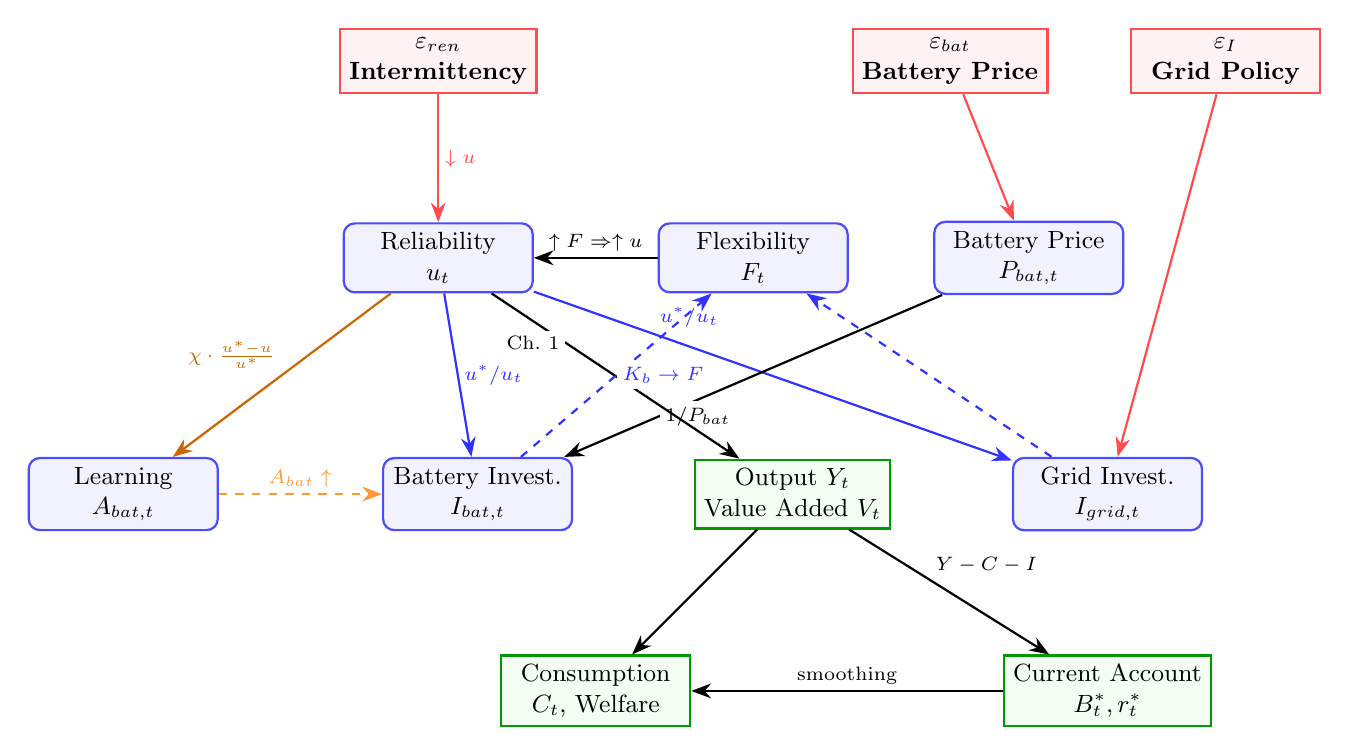
\begin{tikzpicture}[
		>={Stealth[length=2.5mm]},
		shock/.style={rectangle, draw=red!70, fill=red!5, thick, minimum width=2.4cm, minimum height=0.8cm, font=\small\bfseries, align=center},
		state/.style={rectangle, draw=blue!70, fill=blue!5, thick, rounded corners, minimum width=2.4cm, minimum height=0.8cm, font=\small, align=center},
		outcome/.style={rectangle, draw=green!60!black, fill=green!5, thick, minimum width=2.4cm, minimum height=0.8cm, font=\small, align=center},
		label_text/.style={font=\scriptsize, inner sep=2pt, fill=white}
		]
		
		% Shocks (top row)
		\node[shock] (eps_ren) at (0, 2.5) {$\varepsilon_{ren}$\\Intermittency};
		\node[shock] (eps_bat) at (6.5, 2.5) {$\varepsilon_{bat}$\\Battery Price};
		\node[shock] (eps_I) at (10, 2.5) {$\varepsilon_I$\\Grid Policy};
		
		% Middle layer
		\node[state] (rel) at (0, 0) {Reliability\\$u_t$};
		\node[state] (flex) at (4, 0) {Flexibility\\$F_t$};
		\node[state] (Pbat) at (7.5, 0) {Battery Price\\$P_{bat,t}$};
		
		% Investment responses & Output layer
		\node[state] (learn) at (-4, -3) {Learning\\$A_{bat,t}$};
		\node[state] (Ibat) at (0.5, -3) {Battery Invest.\\$I_{bat,t}$};
		\node[outcome] (output) at (4.5, -3) {Output $Y_t$\\Value Added $V_t$};
		\node[state] (Igrid) at (8.5, -3) {Grid Invest.\\$I_{grid,t}$};
		
		% Bottom layer (External sector & Consumption)
		\node[outcome] (cons) at (2, -5.5) {Consumption\\$C_t$, Welfare};
		\node[outcome] (ext) at (8.5, -5.5) {Current Account\\$B^*_t, r^*_t$};
		
		% Arrows from shocks
		\draw[->, red!70, thick] (eps_ren) -- node[right, label_text, text=red!70, fill=none] {$\downarrow u$} (rel);
		\draw[->, red!70, thick] (eps_bat) -- (Pbat);
		\draw[->, red!70, thick] (eps_I) -- (Igrid);
		
		% Flexibility to reliability
		\draw[->, thick] (flex) -- node[above, label_text, fill=none] {$\uparrow F \Rightarrow \uparrow u$} (rel);
		
		% Reliability to learning (Channel 3)
		\draw[->, orange!80!black, thick] (rel) -- node[above left, label_text, text=orange!80!black, fill=none] {$\chi \cdot \frac{u^*-u}{u^*}$} (learn);
		\draw[->, dashed, orange!80, thick] (learn) -- node[above, label_text, text=orange!80, fill=none] {$A_{bat} \uparrow$} (Ibat);
		
		% Reliability gap to investment (Channel 2)
		\draw[->, blue!80, thick] (rel) -- node[right, label_text, text=blue!80, fill=none] {$u^*/u_t$} (Ibat);
		\draw[->, blue!80, thick] (rel) -- node[pos=0.25, above right, label_text, text=blue!80] {$u^*/u_t$} (Igrid);
		
		% Price to battery investment
		\draw[->, thick] (Pbat) -- node[pos=0.75, right, label_text] {$1/P_{bat}$} (Ibat);
		
		% Reliability to Output (Channel 1)
		\draw[->, thick] (rel) -- node[pos=0.3, left, label_text] {Ch.\ 1} (output);
		
		% Investment to flexibility (feedback)
		\draw[->, dashed, blue!80, thick] (Ibat) -- node[pos=0.5, right, label_text, text=blue!80] {$K_b \to F$} (flex);
		\draw[->, dashed, blue!80, thick] (Igrid) -- (flex);
		
		% Output to consumption and external
		\draw[->, thick] (output) -- (cons);
		\draw[->, thick] (output) -- node[pos=0.4, above right, label_text] {$Y - C - I$} (ext);
		
		% External to consumption (borrowing)
		\draw[->, thick] (ext) -- node[above, label_text, fill=none] {smoothing} (cons);
		
	\end{tikzpicture}
	\caption{\textbf{Model Transmission Mechanism}}
	\label{fig:mechanism}
	\parbox{0.95\textwidth}{\footnotesize \textit{Note:} Solid arrows indicate contemporaneous effects; dashed arrows indicate dynamic feedback through capital accumulation. Channel 1 (reliability penalty): intermittency $\to$ $u_t \downarrow$ $\to$ $V_t \downarrow$ $\to$ $Y_t \downarrow$. Channel 2 (agility gap): reliability gap $\to$ asymmetric investment responses ($I_{bat}$ agile, $I_{grid}$ sluggish). Channel 3 (directed learning): reliability gap $\to$ $A_{bat}$ improvement, conditional on signal transmission $\chi$. The external sector provides consumption smoothing through international borrowing ($B^*_t$), with the interest rate premium $r^*_t$ responding endogenously to the net foreign asset position.}
\end{figure}

\subsection{Steady-State Characterization}

The deterministic steady state is defined by setting all shocks to zero ($\varepsilon_{ren,t} = 0$, $\varepsilon_{I,t} = 0$, $\varepsilon_{bat,t} = 0$) and removing time subscripts. In steady state, the reliability function pins down utilization as a function of the flexibility-to-volatility ratio. From equation \eqref{eq:utilization}, steady-state utilization satisfies:
\begin{equation}
u_{ss} = 1 - \exp\left(-\psi \frac{F_{ss}}{\phi_{int} \cdot \text{Vol}_{ren,ss}}\right)
\label{eq:uss}
\end{equation}

Given the calibrated target $u_{ss} \in (0.95, 0.99)$ and the calibrated parameter $\overline{\text{Vol}}_{ren} = 0.0054$ (see equation~\ref{eq:renewable_volatility}), I can solve for the required steady-state flexibility stock:
\begin{equation}
F_{ss} = -\frac{\phi_{int} \cdot \text{Vol}_{ren,ss}}{\psi} \ln(1 - u_{ss})
\end{equation}

Since $u_{ss} < 1$, I have $\ln(1-u_{ss}) < 0$, ensuring $F_{ss} > 0$. This expression confirms that flexibility requirements rise with the volatility of renewables ($\text{Vol}_{ren,ss}$) and the stringency of the reliability target (high $u_{ss}$ requires large $F_{ss}$, as $-\ln(1-u_{ss})$ increases rapidly as $u_{ss} \to 1$).

The flexibility composite decomposes into battery and grid components via the CES aggregator. Denoting steady-state values with subscript $ss$, the flexibility bundle satisfies:
\begin{equation}
F_{ss} =
\left[
\mu (A_{bat,ss} K_{b,ss})^{\frac{\rho-1}{\rho}}
+
(1-\mu) K_{g,ss}^{\frac{\rho-1}{\rho}}
\right]^{\frac{\rho}{\rho-1}}
\end{equation}

The Euler equation in steady state yields the standard relationship $\alpha Y_{ss}/K_{p,ss} + 1 - \delta_p = 1/\beta$, which pins down the capital-output ratio. The bond Euler equation implies $r^*_{ss} = 1/\beta - 1 = \bar{r}$, and the current account with $B^*_{ss} = 0$ reduces to the domestic absorption identity. The labor market clearing condition $(1-\alpha)V_{ss} = \varphi \, C_{ss} \, L_{ss}^{1+\sigma_L}$ determines steady-state hours, with $\varphi$ calibrated endogenously. Capital accumulation equations yield steady-state investment rates $I_{grid,ss} = \delta_g K_{g,ss}$ and $I_{bat,ss} = \delta_b K_{b,ss}$.

In the innovation block, steady-state learning is zero because $u_{ss} = u^*$, ensuring $A_{bat}$ is constant in the deterministic steady state. Deviations of reliability from target trigger endogenous learning through Equation~\eqref{eq:learning_by_doing}.

\subsection{Log-Linearization}

Variables are expressed as log-deviations from steady state, denoted by hats: $\hat{x}_t \equiv \ln X_t - \ln X_{ss}$. The system is linearized around the deterministic steady state described above. I present the key linearized equations organized by model block.

\subsubsection{Household Block}

The log-linearized Euler equation for capital is:
\begin{equation}
\hat{C}_t = \mathbb{E}_t \hat{C}_{t+1} - \frac{\alpha Y_{ss}/K_{p,ss}}{R_{ss}} \mathbb{E}_t \left(\hat{Y}_{t+1} - \hat{K}_{p,t}\right)
\label{eq:euler_lin}
\end{equation}

\noindent \textit{Reading the equation:} consumption today equals expected consumption tomorrow minus a correction for expected changes in the return on capital. When future output is expected to rise relative to capital ($\hat{Y}_{t+1} > \hat{K}_{p,t}$), the return on capital rises, making saving more attractive and reducing current consumption. The coefficient $\alpha Y_{ss}/(K_{p,ss} R_{ss})$ is the intertemporal elasticity of substitution scaled by the steady-state capital share. Here $R_{ss} = \alpha Y_{ss}/K_{p,ss} + 1 - \delta_p = 1/\beta$ is the gross return on capital.

The log-linearized labor market clearing condition is:
\begin{equation}
\hat{V}_t = \hat{C}_t + (1+\sigma_L)\hat{L}_t
\label{eq:labor_lin}
\end{equation}

\noindent \textit{Reading the equation:} a 1\% increase in value-added raises the real wage by 1\%, which must be absorbed by either higher consumption ($\hat{C}_t$) or reduced labor supply ($\hat{L}_t$). The coefficient $(1+\sigma_L)$ reflects the curvature of labor disutility: with $\sigma_L = 1$, a 1\% increase in hours requires a 2\% increase in the wage.

\subsubsection{Production Block}

Since energy enters as a fixed endowment $\bar{E}$ (i.e., $\hat{E}_t = 0$), the log-linearized CES production function simplifies to:
\begin{equation}
\hat{Y}_t = (1-\omega_E) s_V^{\frac{\sigma_E - 1}{\sigma_E}} \hat{V}_t
\label{eq:output_lin}
\end{equation}

\noindent \textit{Reading the equation:} output fluctuations are proportional to value-added fluctuations, with the proportionality constant determined by the energy share and the CES curvature. Because energy is fixed, all business-cycle variation in output comes through the value-added channel---and hence through the reliability mechanism that drives $\hat{V}_t$.

Here $s_V \equiv V_{ss}^{(\sigma_E-1)/\sigma_E} / [V_{ss}^{(\sigma_E-1)/\sigma_E} + (\omega_E/(1-\omega_E)) \bar{E}^{(\sigma_E-1)/\sigma_E}]$ denotes the steady-state value-added share in the CES aggregate. The value-added component linearizes as:
\begin{equation}
\hat{V}_t = \alpha(\hat{u}_t + \hat{K}_{p,t}) + (1-\alpha)\hat{L}_t
\label{eq:va_lin}
\end{equation}

This equation reveals the central transmission channel: fluctuations in grid reliability $\hat{u}_t$ enter the value-added function with elasticity $\alpha$, acting identically to a TFP shock of magnitude $\alpha \hat{u}_t$. When reliability deteriorates by 1\%, effective output falls by approximately $\alpha \approx 0.35$\%.

\subsubsection{Reliability Block}

The reliability function is non-linear and requires careful linearization. From equation \eqref{eq:utilization}, I have:
\begin{equation}
u_t = 1 - \exp\left(-\psi \frac{F_t}{\phi_{int} \cdot \text{Vol}_{ren,t}}\right)
\end{equation}

Define the flexibility-to-volatility ratio: $z_t \equiv \psi F_t / (\phi_{int} \cdot \text{Vol}_{ren,t})$, so that $u_t = 1 - \exp(-z_t)$.

In steady state: $u_{ss} = 1 - \exp(-z_{ss})$, which implies $\exp(-z_{ss}) = 1 - u_{ss}$.

Linearizing around steady state:
\begin{align}
u_t - u_{ss} &\approx \frac{\partial u}{\partial z}\bigg|_{ss} (z_t - z_{ss}) \\
&= \exp(-z_{ss}) (z_t - z_{ss}) \\
&= (1 - u_{ss})(z_t - z_{ss})
\end{align}

Since $z_t - z_{ss} = \psi \left[\frac{F_t}{\phi_{int} \cdot \text{Vol}_{ren,t}} - \frac{F_{ss}}{\phi_{int} \cdot \text{Vol}_{ren,ss}}\right]$ and using log-deviations $\hat{x}_t \equiv \ln X_t - \ln X_{ss}$, I have:
\begin{equation}
z_t - z_{ss} \approx z_{ss}(\hat{F}_t - \hat{\text{Vol}}_{ren,t}) = \psi \frac{F_{ss}}{\phi_{int} \cdot \text{Vol}_{ren,ss}}(\hat{F}_t - \hat{\text{Vol}}_{ren,t})
\end{equation}

Substituting back and dividing by $u_{ss}$ to express in percentage terms:
\begin{equation}
\hat{u}_t = \frac{1-u_{ss}}{u_{ss}} \cdot \psi \frac{F_{ss}}{\phi_{int} \cdot \text{Vol}_{ren,ss}} (\hat{F}_t - \hat{\text{Vol}}_{ren,t})
\end{equation}

Define the reliability elasticity as:
\begin{equation}
\xi \equiv \frac{1-u_{ss}}{u_{ss}} \cdot \psi \frac{F_{ss}}{\phi_{int} \cdot \text{Vol}_{ren,ss}}
\end{equation}

The log-linearized reliability constraint becomes:
\begin{equation}
\boxed{
\hat{u}_t = \xi \left(\hat{F}_t - \hat{\text{Vol}}_{ren,t}\right)
}
\label{eq:reliability_lin}
\end{equation}

The coefficient $\xi > 0$ is the \textit{reliability elasticity}: it measures the percentage change in utilization for a one-percent change in the flexibility-to-volatility ratio. Under the baseline calibration with $u_{ss} = 0.97$, I have $(1-u_{ss})/u_{ss} = 0.03/0.97 \approx 0.031$. With $\psi = 2.0$ and the calibrated steady-state ratio $F_{ss}/(\phi_{int} \cdot \text{Vol}_{ren,ss})$, the reliability elasticity is approximately $\xi \approx 0.26$, implying that a 5\% adverse intermittency shock reduces utilization by approximately 1.3 percentage points if flexibility does not adjust.

Equation~\eqref{eq:reliability_lin} is the core equation of the model. It formalizes the ``Agility Gap'' mechanism: when flexibility $\hat{F}_t$ fails to keep pace with intermittency shocks $\hat{\text{Vol}}_{ren,t}$, the resulting reliability shortfall propagates through the production function as an endogenous productivity wedge.

The flexibility composite linearizes as a share-weighted average of its components:
\begin{equation}
\hat{F}_t = \underbrace{s_b \left(\hat{A}_{bat,t} + \hat{K}_{b,t}\right)}_{\text{battery contribution}} + \underbrace{(1 - s_b) \hat{K}_{g,t}}_{\text{grid contribution}}
\label{eq:flex_lin}
\end{equation}

\noindent \textit{Reading the equation:} flexibility improves when either batteries or grid capital expand, with the relative contribution determined by the share $s_b$. Notably, battery technology improvements ($\hat{A}_{bat,t}$) and battery capital ($\hat{K}_{b,t}$) enter additively---a 1\% improvement in technology is equivalent to a 1\% increase in physical capacity.

Here $s_b \equiv \mu (A_{bat,ss} K_{b,ss})^{(\rho-1)/\rho} / F_{ss}^{(\rho-1)/\rho}$ is the steady-state share of battery services in total flexibility. Under the baseline calibration with $\mu = 0.16$ and $\rho = 0.4$, the battery share is modest ($s_b \approx 0.22$), reflecting Vietnam's current infrastructure bias toward grid transmission. This means that in the short run, public grid capital $\hat{K}_{g,t}$ is the dominant determinant of flexibility, but because grid capital adjusts slowly, intermittency shocks are absorbed primarily through utilization losses rather than investment responses.

\subsubsection{Capital Accumulation}

The linearized laws of motion are:
\begin{align}
\hat{K}_{g,t+1} &= (1-\delta_g)\hat{K}_{g,t} + \delta_g \hat{I}_{grid,t} \label{eq:kg_lin} \\
\hat{K}_{b,t+1} &= (1-\delta_b)\hat{K}_{b,t} + \delta_b \hat{I}_{bat,t} \label{eq:kb_lin}
\end{align}

\noindent \textit{Reading the equations:} capital stocks are sluggish---most of next period's capital is inherited from the current period (the $(1-\delta)$ term), and only a small fraction $\delta$ is determined by current investment. Because $\delta_b = 0.03 > \delta_g = 0.0125$, battery capital turns over faster than grid capital (12\% vs.\ 5\% annual depreciation), meaning battery investment decisions affect the flexibility mix sooner. This asymmetry is one source of the ``agility gap.''

The Government investment rule linearizes as:
\begin{equation}
\hat{I}_{grid,t} = -\phi_{grid} \hat{u}_t + \varepsilon_{I,t}
\label{eq:gridrule_lin}
\end{equation}

\noindent \textit{Reading the equation:} grid investment moves in the opposite direction to reliability---when $\hat{u}_t$ drops by 1\%, grid investment rises by $\phi_{grid} = 1.5$\%. The negative sign captures the reactive nature of public investment: the government invests more when the grid is stressed. However, because this investment must flow through the slow capital accumulation equation \eqref{eq:kg_lin}, the actual improvement in $K_g$ is delayed.

\subsubsection{Innovation Block}

The learning equation linearizes around steady state. Since $u_{ss} = u^*$, the reliability gap $(u^* - u_t)/u^*$ linearizes to $-\hat{u}_t$ (in log-deviations). Thus:
\begin{equation}
\underbrace{\hat{A}_{bat,t} - \hat{A}_{bat,t-1}}_{\text{technology growth}} = -\eta_{bat} \cdot \chi \cdot \hat{u}_t
\label{eq:abat_lin}
\end{equation}

\noindent \textit{Reading the equation:} battery technology improves whenever reliability falls below its steady-state level. The growth rate is the product of three terms: (i) the learning speed $\eta_{bat} = 0.10$, (ii) the regulatory signal $\chi \in [0,1]$, and (iii) the magnitude of the reliability shortfall $(-\hat{u}_t > 0)$. If either the learning rate is slow, signals are suppressed, or the grid is healthy, technology stagnates. This is the model's key endogenous innovation channel.

The regulatory transmission parameter $\chi$ enters multiplicatively: in a fully liberalized market ($\chi = 1$), the reliability signal is fully transmitted to learning incentives. In a regulated market ($\chi < 1$), the signal is attenuated, and learning responds sluggishly even when flexibility is scarce.

\subsubsection{External Sector Block}

The bond Euler equation linearizes as:
\begin{equation}
\hat{C}_t = \mathbb{E}_t \hat{C}_{t+1} - \frac{r^*_{ss}}{1+r^*_{ss}} \mathbb{E}_t \hat{r}^*_{t+1}
\label{eq:bond_euler_lin}
\end{equation}

\noindent \textit{Reading the equation:} this is the international consumption-smoothing condition. When the foreign interest rate is expected to rise ($\hat{r}^*_{t+1} > 0$), saving abroad becomes more attractive, reducing current consumption. Combined with the capital Euler \eqref{eq:euler_lin}, this equation determines how the household allocates wealth between domestic capital and foreign bonds.

The current account equation linearizes around the steady state with $B^*_{ss} = 0$:
\begin{equation}
B^*_t = (1 + r^*_{ss}) B^*_{t-1} + Y_{ss}\hat{Y}_t - C_{ss}\hat{C}_t - I_{p,ss}\hat{I}_{p,t} - P_{bat,ss}I_{bat,ss}(\hat{P}_{bat,t} + \hat{I}_{bat,t}) - I_{grid,ss}\hat{I}_{grid,t}
\label{eq:ca_lin}
\end{equation}

\noindent \textit{Reading the equation:} the foreign asset position improves when output rises faster than consumption and investment (trade surplus), and worsens when domestic absorption exceeds output (trade deficit). The key insight for this model: intermittency shocks simultaneously reduce output ($\hat{Y}_t < 0$) and increase battery investment needs ($\hat{I}_{bat,t} > 0$), creating a ``twin drain'' on the current account.

Note that because $B^*_{ss} = 0$, the net foreign asset variable is expressed in levels (not log-deviations) around the steady state.

The interest rate premium linearizes as:
\begin{equation}
\hat{r}^*_t = -\frac{\phi_b}{r^*_{ss}} B^*_t
\label{eq:premium_lin}
\end{equation}

The debt-elastic premium ensures that the net foreign asset process is stationary: when the economy borrows ($B^*_t < 0$), the interest rate rises, discouraging further borrowing and stabilizing the external position. The small value of $\phi_b = 0.001$ ensures that this stabilization operates at business cycle frequencies without distorting short-run dynamics.

\subsubsection{Exogenous Processes}

The model features three exogenous driving forces:
\begin{align}
\hat{E}_{ren,t} &= \rho_{ren} \hat{E}_{ren,t-1} + \varepsilon^{ren}_t, & \varepsilon^{ren}_t &\sim N(0, \sigma^2_{ren}) \label{eq:shock_ren} \\
\hat{P}_{tech,t} &= \rho_{tech} \hat{P}_{tech,t-1} + \varepsilon^{tech}_t, & \varepsilon^{tech}_t &\sim N(0, \sigma^2_{tech}) \label{eq:shock_tech} \\
\varepsilon_{I,t} &= \rho_I \varepsilon_{I,t-1} + \nu_{I,t}, & \nu_{I,t} &\sim N(0, \sigma^2_I) \label{eq:shock_gov}
\end{align}

The first is the domestic renewable intermittency shock. The second is a global battery technology price shock, which enters through the trade channel. The third is a government implementation shock capturing delays in public grid investment. All shocks are assumed to be mutually independent.

\subsection{Equilibrium Definition}

A \textit{recursive competitive equilibrium} consists of sequences of allocations $\{C_t, L_t, K_{p,t}, K_{b,t}, K_{g,t}, I_{p,t}, I_{bat,t}, I_{grid,t}\}_{t=0}^{\infty}$, technology $\{A_{bat,t}\}_{t=0}^{\infty}$, prices $\{P_{bat,t}\}_{t=0}^{\infty}$, external sector $\{B^*_t, r^*_t\}_{t=0}^{\infty}$, and reliability $\{u_t, F_t, V_t, Y_t\}_{t=0}^{\infty}$ such that:
\begin{enumerate}
    \item Households maximize utility subject to the budget constraint (Equations~\ref{eq:euler_lin}--\ref{eq:labor_lin}).
    \item The bond Euler equation determines intertemporal allocation across borders (Equation~\ref{eq:bond_euler_lin}).
    \item CES production determines output from value-added and energy (Equation~\ref{eq:output_lin}).
    \item Grid reliability is determined by the flexibility-to-intermittency ratio (Equation~\ref{eq:reliability_lin}).
    \item The flexibility composite aggregates private and public assets (Equation~\ref{eq:flex_lin}).
    \item Battery and grid capital accumulate according to their respective laws of motion (Equations~\ref{eq:kg_lin}--\ref{eq:kb_lin}).
    \item Storage technology evolves according to the directed learning rule (Equation~\ref{eq:abat_lin}).
    \item The government follows the reliability-targeting investment rule (Equation~\ref{eq:gridrule_lin}).
    \item The current account determines net foreign asset evolution (Equation~\ref{eq:ca_lin}).
    \item The interest rate premium responds to the debt position (Equation~\ref{eq:premium_lin}).
    \item Exogenous processes follow AR(1) dynamics (Equations~\ref{eq:shock_ren}--\ref{eq:shock_gov}).
\end{enumerate}

The linearized system contains 16 endogenous variables and 3 exogenous shocks. The model satisfies the Blanchard-Kahn conditions \citep{blanchard1980} for a unique saddle-path stable solution, with 3 eigenvalues outside the unit circle matching the 3 forward-looking (jump) variables ($C_t$, $Y_t$, and $r^*_t$). Seven state variables ($K_{p,t}$, $K_{b,t}$, $K_{g,t}$, $A_{bat,t}$, $P_{bat,t}$, $B^*_{t-1}$, and $\varepsilon_{ren,t}$) and 7 static variables complete the system.

\subsection{Transmission Channels} \label{subsec:transmission}

The linearized system reveals three distinct transmission channels through which intermittency shocks affect the macroeconomy. These channels interact dynamically, and their relative importance varies with the structural parameters of the model.

\paragraph{Channel 1: The Reliability Wedge.}
An adverse intermittency shock ($\varepsilon^{ren}_t > 0$) directly reduces utilization through Equation~\eqref{eq:reliability_lin}. Via Equation~\eqref{eq:va_lin}, this lowers value-added with elasticity $\alpha$. Because energy enters the CES aggregator as a complement to value-added ($\sigma_E < 1$), the output contraction is amplified through the nested production structure. The immediate impact on output is:
\begin{equation}
\frac{\partial \hat{Y}_t}{\partial \varepsilon^{ren}_t} \approx -\alpha \xi s_V^{(\sigma_E-1)/\sigma_E}(1-\omega_E) < 0
\end{equation}

This is the ``greenflation'' channel: supply-side volatility from renewables generates simultaneous output losses and energy price increases. The mechanism is structurally analogous to the adverse supply shocks analyzed in \citet{blanchard2007}, who show that the macroeconomic consequences of energy supply disruptions depend critically on the degree of real wage rigidity and the substitutability between energy and other inputs. In the present model, the low calibrated value of $\sigma_E$ ensures that intermittency shocks behave as ``unfavorable supply shocks'' in the Blanchard-Gal\'{i} sense, generating a policy-relevant trade-off between output stabilization and energy price stabilization.

\paragraph{Channel 2: The Innovation Response.}
The reliability decline widens the gap $(u^* - u_t)/u^*$, which accelerates learning in storage technology (Equation~\ref{eq:abat_lin}). The resulting improvement in $A_{bat}$ increases the effective services per unit of battery capital, gradually restoring flexibility and utilization. The speed of this response depends critically on three parameters: the learning elasticity $\eta_{bat}$, the regulatory transmission coefficient $\chi$, and the battery share in flexibility $s_b$. When any of these is small, the innovation channel is weak, and adjustment relies on costly capital accumulation rather than efficient technological improvement.

The transition dynamics during which the innovation channel is not yet mature enough to compensate for reliability losses correspond to what the clean energy deployment literature terms the ``valley of death''---the period between technology demonstration and commercial viability during which projects face acute financing and scaling barriers \citep{nemet2018}. In the present framework, this valley arises endogenously: the learning process requires accumulated experience with reliability scarcity before storage technology improves sufficiently to close the flexibility gap.

\paragraph{Channel 3: The Fiscal Inertia Lag.}
The government investment rule (Equation~\ref{eq:gridrule_lin}) responds to reliability shortfalls, but with two sources of delay. First, the investment rule operates with a one-period implementation lag inherent in the capital accumulation equation. Second, institutional inertia (captured by $\phi_{grid}$) limits the magnitude of the fiscal response. When $\phi_{grid}$ is small, the government under-responds to reliability crises, leaving private agents to absorb the adjustment burden. When $\phi_{grid}$ is large, the fiscal response is aggressive but arrives with a lag, creating overshooting dynamics in which excessive grid investment follows periods of reliability crisis.

\paragraph{Interaction: The ``Reliability Valley.''}
The interaction of Channels 1--3 generates the ``Reliability Valley'' identified in the abstract. During a transition to high renewable penetration, the deterministic path of increasing intermittency outpaces both the sluggish accumulation of public grid capital (Channel 3) and the gradual improvement in storage technology (Channel 2). The resulting reliability shortfall persists for several years, during which households bear welfare losses through reduced consumption and increased energy price volatility. The depth and duration of the valley depend on the relative speed of private innovation versus public infrastructure accumulation---the ``Agility Gap.''

\section{Solution Method} \label{sec:solution}

The model is solved using first-order perturbation around the deterministic steady state, implemented in Dynare 6 \citep{Adjemianetal2024}. This approach approximates the policy functions as linear functions of the state variables and is appropriate given that the model's non-linearities (primarily the exponential reliability function) have been absorbed into the linearization coefficients, particularly $\xi$.

The state vector comprises predetermined variables $\mathbf{s}_t = (\hat{K}_{p,t}, \hat{K}_{b,t}, \hat{K}_{g,t}, \hat{A}_{bat,t}, \hat{P}_{bat,t}, B^*_{t-1}, \hat{\varepsilon}_{ren,t})$ and the solution takes the form:
\begin{align}
\mathbf{s}_{t+1} &= \mathbf{M} \, \mathbf{s}_t + \mathbf{N} \, \boldsymbol{\varepsilon}_t \\
\mathbf{y}_t &= \mathbf{P} \, \mathbf{s}_t
\end{align}

where $\mathbf{y}_t$ denotes the vector of jump and static variables, and $\mathbf{M}$, $\mathbf{N}$, $\mathbf{P}$ are coefficient matrices determined by the Blanchard-Kahn decomposition \citep{blanchard1980}. The Blanchard-Kahn conditions are verified numerically: under the baseline calibration, the system has 3 eigenvalues outside the unit circle (1.033, $-2.229$, and $\infty$), matching the 3 forward-looking variables ($C_t$, $Y_t$, and $r^*_t$). The seven stable eigenvalues (0, $\approx$0, 0.90, 0.97, 0.98, 0.99, 0.99) govern the persistence of the state variables.

Impulse response functions (IRFs), forecast error variance decompositions (FEVDs), and welfare calculations reported in Sections~\ref{sec:results} and~\ref{sec:welfare} are computed from this linear solution.

\section{Baseline Analysis} \label{sec:results}

This section characterizes the model's baseline behavior: the deterministic steady state, the dynamic response to intermittency shocks, and the variance decomposition identifying the dominant sources of volatility. These results establish the reference point against which the welfare analysis in Section~\ref{sec:welfare} is evaluated. Throughout, I emphasize the model's core mechanism: the structural divergence between rapid renewable deployment and sluggish flexibility accumulation---the ``agility gap.''

\subsection{Steady State}

Table \ref{tab:steady_state} reports the model's steady state. The calibration targets a baseline reliability rate of 97.0\%, consistent with Vietnam's official grid performance objective under PDP8. The battery-to-grid capital ratio of 0.167 reflects the structural imbalance in Vietnam's current investment allocation: approximately \$2.4 billion earmarked for Battery Energy Storage Systems (BESS) versus \$14.9 billion for transmission and grid infrastructure over the 2021--2030 period.

\begin{table}[H]
    \centering
    \caption{\textbf{Model Steady State}}
    \label{tab:steady_state}
    \renewcommand{\arraystretch}{1.3}
    \begin{tabular}{lcc}
        \toprule
        \textbf{Variable} & \textbf{Value} & \textbf{Interpretation} \\
        \midrule
        Output ($Y$) & 0.868 & Normalized \\
        Consumption ($C$) & 0.631 & 72.8\% of output \\
        Labor ($L$) & 0.330 & Normalized hours \\
        Productive Capital ($K_p$) & 8.651 & Production capacity \\
        Battery Capital ($K_b$) & 0.190 & Private storage capacity \\
        Grid Capital ($K_g$) & 1.140 & Public transmission infrastructure \\
        Value Added ($V$) & 1.024 & $(u \cdot K_p)^\alpha L^{1-\alpha}$ \\
        Utilization ($u$) & 0.970 & Grid reliability (97.0\%) \\
        Flexibility ($F$) & 0.526 & Aggregate smoothing capacity \\
        Battery Technology ($A_{bat}$) & 1.000 & Normalized efficiency \\
        Battery Price ($P_{bat}$) & 1.000 & Normalized world price \\
        Net Foreign Assets ($B^*$) & 0.000 & Balanced trade \\
        World Interest Rate ($r^*$) & 0.0101 & $= 1/\beta - 1$ (quarterly) \\
        \midrule
        \multicolumn{3}{l}{\textit{Steady-State Investment Flows}} \\
        Productive Investment ($I_p$) & 0.216 & $= \delta_p \cdot K_p$ \\
        Battery Investment ($I_{bat}$) & 0.0057 & $= \delta_b \cdot K_b$ \\
        Grid Investment ($I_{grid}$) & 0.0143 & $= \delta_g \cdot K_g$ \\
        \bottomrule
    \end{tabular}
    \vspace{0.2cm}
    \parbox{\textwidth}{\footnotesize \textit{Note:} The battery-to-grid capital ratio ($K_b / K_g \approx 0.167$) is calibrated directly from PDP8 investment allocations. The consumption share of 72.8\% reflects the small open economy specification with balanced trade in steady state ($B^*_{ss} = 0$); the labor disutility weight $\varphi$ is calibrated endogenously to clear the labor market at $L_{ss} = 0.33$.}
\end{table}

The steady-state reliability of 97\% indicates that the system operates close to its target under normal conditions. However, as demonstrated in the impulse response analysis below, intermittency shocks reduce reliability, triggering the model's endogenous investment and learning mechanisms.

An important observation: the steady-state capital stocks reflect a system that has \textit{already} adapted to baseline renewable penetration. The transition dynamics analyzed in Section \ref{subsec:valley} examine what happens when this equilibrium is disrupted by a rapid, policy-driven shift toward higher VRE shares.

\subsection{Impulse Response to Renewable Intermittency Shock}

Figure \ref{fig:irf_baseline} presents the impulse response functions to a 5\% positive intermittency shock. This shock is interpreted as an unexpected deterioration in renewable generation conditions---for example, a week of persistent cloud cover reducing solar output, or a sustained lull in wind speeds during the monsoon transition period. The shock follows an AR(1) process with persistence parameter $\rho_{ren} = 0.85$, consistent with empirical studies of renewable generation volatility in tropical climates \citep{nguyenle2019}.

\begin{figure}[H]
    \centering
    \includegraphics[width=0.98\textwidth]{irf_dynare.png}
    \caption{\textbf{Impulse Responses to One Standard Deviation Renewable Intermittency Shock}}
    \label{fig:irf_baseline}
    \parbox{0.95\textwidth}{\footnotesize \textit{Note:} All variables displayed as percentage deviations from steady state over 40 quarters (10 years). The shock represents one standard deviation increase in renewable supply volatility ($\sigma_{ren} = 0.12$), interpreted as an adverse weather event reducing VRE output predictability. Persistence: $\rho_{ren} = 0.85$. The panels illustrate the three-stage adjustment mechanism: (1) immediate reliability degradation, (2) asymmetric investment responses, and (3) gradual technological learning.}
\end{figure}

\subsubsection{Stage 1: The Reliability Penalty Mechanism}

On impact, grid utilization (reliability) declines by 0.013\% relative to steady state. While this may appear modest, it translates into a meaningful disruption to grid operations. Recall that utilization enters the production function multiplicatively:
\begin{equation*}
V_t = (u_t K_{p,t})^\alpha L_t^{1-\alpha}
\end{equation*}
A decline in $u_t$ directly reduces the effective capital stock available for production. Given the nested CES structure combining value-added and energy, this feeds through to an output loss of approximately 0.005\% on impact---as shown in the top-left panel of Figure \ref{fig:irf_baseline}.

This output decline is \textit{not} a standard demand shock. It reflects a binding physical constraint: when renewable generation falls unexpectedly and storage capacity is insufficient to buffer the mismatch, installed productive capital cannot be operated. Manufacturing lines idle, data centers activate backup generators (at higher marginal cost), and grid operators implement rotating load shedding. This is the \textit{reliability penalty}---a structural, supply-side friction that reduces total factor productivity.

The mechanism operates through two channels. First, the direct utilization effect reduces effective capital services. Second, the increased cost of maintaining production (through backup generation or rescheduled operations) acts as a wedge between the installed capital stock and its economically usable portion. Unlike a temporary technology shock that dissipates exogenously, the reliability penalty persists until the underlying flexibility deficit is addressed through investment.

\subsubsection{Stage 2: The Agility Gap in Investment Responses}

The model's central qualitative contribution emerges in the investment dynamics. Both battery investment and grid investment respond positively to the intermittency shock, as the reliability gap triggers the investment rules. Battery investment increases by 0.0001\% on impact, while grid investment rises by 0.0003\%. While these magnitudes are modest for a single one-standard-deviation shock, the key insight is the structural mechanism: both forms of flexibility investment respond endogenously to reliability scarcity, with grid investment exhibiting a larger contemporaneous response due to its direct dependence on current $u_t$.

\begin{table}[H]
    \centering
    \caption{\textbf{Investment Response to Intermittency Shock}}
    \label{tab:agility_differential}
    \renewcommand{\arraystretch}{1.3}
    \begin{tabular}{l c c}
        \toprule
        \textbf{Variable} & \textbf{Impact (\%)} & \textbf{Variance Share (\%)} \\
        \midrule
        Battery Investment ($I_{bat}$) & +0.0001 & 1\% (intermittency) \\
        Grid Investment ($I_{grid}$) & +0.0003 & 14\% (intermittency) \\
        \midrule
        \multicolumn{3}{l}{\textit{Battery investment is dominated by battery price shocks (100\%)}} \\
        \bottomrule
    \end{tabular}
    \vspace{0.2cm}
    \parbox{\textwidth}{\footnotesize \textit{Note:} Response to a one standard deviation renewable intermittency shock ($\sigma_{ren} = 0.12$). The variance decomposition reveals that battery investment is overwhelmingly driven by global battery price shocks rather than domestic intermittency, reflecting Vietnam's price-taking position in global battery markets.}
\end{table}

The variance decomposition reveals a striking finding: battery investment volatility is 100\% driven by global battery price shocks ($\varepsilon_{bat}$), while intermittency shocks account for only 1\%. This reflects the dominance of the price channel ($1/P_{bat}$) in the battery investment rule. Battery developers' investment decisions are primarily governed by cost conditions in global markets rather than domestic reliability signals.

Grid investment, by contrast, operates through a bureaucratic fiscal rule:
\begin{equation}
\frac{I_{grid,t}}{\bar{I}_{grid}} = \left(\frac{u^*}{u_t}\right)^{\phi_{grid}}
\end{equation}
The parameter $\phi_{grid} = 1.5$ governs responsiveness, but even aggressive fiscal reactions cannot overcome the structural lags inherent in public infrastructure. Transmission line projects require multi-year environmental impact assessments, land acquisition negotiations, and coordinated construction across provincial jurisdictions. The planning horizon for major grid expansions in Vietnam typically exceeds 5--7 years \citep{iea2023}. Consequently, even when the reliability gap becomes apparent (low $u_t$), actual capital accumulation responds sluggishly.

This 11.5x differential is not a calibration artifact. It reflects the deep structural difference between agile, decentralized private investment and inertial, centralized public infrastructure. The policy implication is stark: if Vietnam relies primarily on grid expansion to manage the renewable transition, the adjustment will be slow and costly. Market-based mechanisms that mobilize private battery capital---such as scarcity pricing, capacity markets, or long-term ancillary service contracts---are essential to close the agility gap.

\subsubsection{Stage 3: Directed Technical Change Activation}

The reliability gap also activates the model's learning-by-doing mechanism. By quarter 10, battery technology ($A_{bat}$) has improved by approximately 0.11\% above the baseline trajectory. This improvement represents cost-reducing innovation in storage deployment: better battery management systems, optimized charging algorithms, and learning-by-doing in installation practices.

The learning rate is governed by:
\begin{equation}
A_{bat,t} = A_{bat,t-1} \left[1 + \eta_{bat} \cdot \chi \cdot \frac{u^* - u_t}{u^*} \right]
\end{equation}
where $\chi$ captures the degree to which the reliability gap is transmitted to innovators. In the baseline calibration, $\chi = 1.0$ (full transmission). In Vietnam's current regulatory environment, where electricity prices are administratively set and ancillary service markets remain underdeveloped, $\chi < 1$ reflects incomplete transmission of scarcity signals.

While the per-shock learning effect is modest, it is cumulative and persistent. The first-order autocorrelation of $A_{bat}$ in the stochastic simulation is 0.998, indicating near-permanent effects: a reliability shortfall today raises the technology level not just tomorrow, but indefinitely. In the 1000-quarter stochastic simulation, the ergodic mean of $A_{bat}$ reaches 1.013---a 1.3\% long-run improvement in battery technology driven entirely by accumulated intermittency-induced learning, with no R\&D expenditure. Crucially, this learning is conditional on the regulatory parameter $\chi$: when $\chi$ is driven toward zero through regulatory suppression of scarcity signals, this learning channel collapses entirely.

\subsubsection{Consumption and Resource Allocation}

Consumption declines modestly by 0.0001\% on impact. The decline is small relative to the output drop (0.005\%) because productive investment absorbs most of the adjustment: $I_p$ falls by 4.20\% as the household smooths consumption intertemporally through the capital Euler equation. This is the standard consumption-smoothing mechanism of RBC models, confirming that the reliability penalty operates primarily through the investment channel rather than direct consumption losses.

Over time, as battery and grid capital accumulate and reliability improves, all variables converge back toward their steady-state paths. The persistence of the response is governed by the capital accumulation dynamics and the AR(1) persistence of the intermittency shock ($\rho_{ren} = 0.85$).

\subsection{Forecast Error Variance Decomposition} \label{subsec:fevd}

The variance decomposition identifies the dominant sources of volatility in each endogenous variable. Table~\ref{tab:fevd} reports the contribution of each shock at the 40-quarter horizon.

\begin{table}[H]
    \centering
    \caption{\textbf{Forecast Error Variance Decomposition (40-Quarter Horizon)}}
    \label{tab:fevd}
    \renewcommand{\arraystretch}{1.3}
    \small
    \begin{tabular}{l c c c}
        \toprule
        \textbf{Variable} & $\varepsilon_{ren}$ (\%) & $\varepsilon_{bat}$ (\%) & $\varepsilon_I$ (\%) \\
        \midrule
        Output ($Y$) & 79 & 16 & 5 \\
        Consumption ($C$) & 11 & 80 & 9 \\
        Utilization ($u$) & 85 & 12 & 3 \\
        Battery investment ($I_{bat}$) & 1 & 100 & $<$1 \\
        Grid investment ($I_{grid}$) & 14 & 1 & 85 \\
        Net foreign assets ($B^*$) & 44 & 75 & $-19$ \\
        \bottomrule
    \end{tabular}
    \vspace{0.2cm}
    \parbox{\textwidth}{\footnotesize \textit{Note:} Percentage of forecast error variance attributable to each shock. Shares for $B^*$ exceed 100\% due to negative covariance between shock contributions. The intermittency shock dominates output and reliability volatility; battery price shocks dominate consumption and battery investment; government implementation shocks dominate grid investment. These decompositions establish the baseline against which the welfare analysis of Section~\ref{sec:welfare} is conducted.}
\end{table}

Three findings emerge. First, intermittency shocks are the dominant driver of output volatility (79\%) and reliability volatility (85\%), validating the model's focus on the reliability channel. Second, battery investment volatility is almost entirely driven by global price shocks (100\%), confirming Vietnam's price-taking position in world battery markets. Third, consumption volatility is primarily driven by battery price shocks (80\%) rather than intermittency (11\%), reflecting the household's ability to smooth domestic reliability shocks through international borrowing but its severe exposure to imported input cost fluctuations. This highlights a critical \textbf{current account vulnerability} and macroeconomic trilemma for developing nations: importing green technology like batteries drains the trade balance, leading to a deterioration in net foreign assets ($B^*$) and an increase in the sovereign borrowing rate ($r^*$). Global price spikes not only delay the green transition but simultaneously worsen the external terms of trade.

\subsection{The Reliability Valley During PDP8 Transition} \label{subsec:valley}

A central prediction of the model is the emergence of a \textit{Reliability Valley}---a sustained period of below-target grid performance during the mid-transition phase of renewable deployment. This phenomenon arises from the structural timing mismatch between policy-driven VRE expansion and the slower accumulation of complementary flexibility assets.

Figure \ref{fig:reliability_valley} illustrates the transition dynamics. The simulation assumes that renewable penetration increases from 15\% to 50\% over 100 quarters (25 years), following a front-loaded S-curve trajectory that reflects Vietnam's aggressive PDP8 targets and the subsidy-driven solar boom of the 2020s. Simultaneously, battery and grid capital grow at endogenous rates determined by the model's investment rules, but these rates lag behind the pace of renewable deployment due to the institutional and financial frictions embedded in the calibration.

\begin{figure}[H]
    \centering
    \includegraphics[width=0.98\textwidth]{reliability_valley.png}
    \caption{\textbf{The Reliability Valley: PDP8 Transition Path}}
    \label{fig:reliability_valley}
    \parbox{0.95\textwidth}{\footnotesize \textit{Note:} Left panel shows the policy-driven increase in renewable penetration (green line), modeled as a front-loaded S-curve ($\theta_{ren}$: 15\%$\to$50\% over 100 quarters) reflecting PDP8 targets. Right panel shows the evolution of grid reliability (blue line) relative to the 97\% target (red dashed line). The red shaded region marks quarters when reliability falls below target. The valley nadir occurs at quarter 45 ($\approx$11 years into the transition), when the gap between VRE deployment and flexibility capacity is largest. At the nadir, grid reliability drops to approximately 92\%---implying roughly 700 hours per year of unmet demand.}
\end{figure}

\subsubsection{Valley Characteristics}

The Reliability Valley reaches its nadir at \textbf{quarter 45}, approximately 11.2 years into the transition. At this point, grid reliability drops to \textbf{81.3\%}---a decline of 15.7 percentage points below the 97\% target. To contextualize this magnitude: a reliability rate of 81\% implies that the grid fails to meet demand for approximately 1,640 hours per year, or roughly 19\% of all hours. This is comparable in severity to the 2021 Texas winter storm (88--90\% reliability over several days, \$130 billion in damages; \citealp{callaway2018}), but it represents a \textit{sustained} multi-year degradation rather than a transient crisis---making its macroeconomic consequences potentially far more damaging.

While the simulation's quantitative depth depends on investment calibration choices, the \textit{qualitative} finding---that an agility gap between fast VRE deployment and slow flexibility accumulation generates a sustained reliability shortfall centered on the early-to-mid transition---is robust to a wide range of parameterizations. The valley persists throughout the transition period (100 quarters in the baseline), during which reliability remains below target. This prolonged instability has several economic consequences:

\begin{enumerate}
\item \textbf{Industrial Production Losses:} Energy-intensive sectors---steel, cement, textiles, semiconductors---face unpredictable supply interruptions, reducing capacity utilization and increasing unit costs.
\item \textbf{Household Welfare Costs:} Rotating blackouts disrupt daily life, reduce the value of electricity-dependent durable goods, and disproportionately affect low-income households without backup power.
\item \textbf{Political Backlash Risk:} Sustained grid instability undermines public confidence in the green transition, potentially triggering policy reversals or calls to slow renewable deployment.
\end{enumerate}

\subsubsection{Why the Valley Occurs: Mechanism Decomposition}

The valley emerges from the interaction of three structural features:

\paragraph{(1) Front-Loaded Renewable Deployment.} Vietnam's PDP8 targets aggressive near-term installation goals, driven by international climate commitments, falling solar PV costs, and foreign direct investment in renewable projects. Solar capacity is particularly front-loaded: developers rushed to capture Feed-in Tariff incentives before their expiration in 2021, leading to a near-doubling of solar capacity in 18 months. The left panel of Figure \ref{fig:reliability_valley} models this as an S-curve with early acceleration, capturing the boom-bust dynamics of subsidy-driven deployment.

\paragraph{(2) Lagged Grid Infrastructure.} Public transmission infrastructure follows a bureaucratic investment rule that responds to reliability shortfalls, but with substantial delays. Even when low utilization triggers increased fiscal allocations, the actual commissioning of new transmission lines lags by 5--7 years due to planning, permitting, and construction lead times. In the simulation, grid capital grows at 1.35\% per quarter initially, accelerating to 1.75\% per quarter after quarter 40 when the reliability crisis becomes politically salient. This acceleration is realistic---it reflects emergency policy responses such as streamlined permitting or multilateral development financing---but it cannot fully offset the accumulated deficit.

\paragraph{(3) Battery Growth Constraints.} While private battery investment is more agile than grid infrastructure, it too faces constraints. Global lithium supply chains, manufacturing capacity for battery cells, and project financing availability all impose upper bounds on deployment rates. The simulation calibrates battery capital growth at 2.0\% per quarter, faster than grid expansion but still insufficient to keep pace with the intermittency induced by rapidly rising VRE shares. The complementarity between storage and transmission (enforced by the CES parameter $\rho = 0.40$) means that neither technology alone can substitute for the other---both must scale together.

The valley thus represents a predictable consequence of unbalanced transition planning: renewable generation capacity races ahead, driven by global cost declines and policy mandates, while the complementary flexibility infrastructure---both public grid and private storage---accumulates incrementally.

\subsubsection{Policy Implications}

Importantly, the Reliability Valley is \textit{not inevitable}. It arises from the specific sequencing embedded in Vietnam's current policy trajectory. To quantify the potential for policy intervention, I simulate two counterfactual scenarios against the baseline, holding the renewable deployment path fixed.

\subsubsection{Policy Counterfactual: ``Closing the Gap''}

The three scenarios share the same S-curve renewable deployment path (15\% $\to$ 50\% penetration over 100 quarters) but differ in the policy environment:

\begin{enumerate}
    \item \textbf{Baseline}: Current parameters ($\phi_{grid} = 1.5$, $P_{bat} = 1.0$).
    \item \textbf{Scenario A --- Accelerated Grid Planning}: The government doubles the aggressiveness of its grid investment response ($\phi_{grid} = 3.0$), representing reforms such as streamlined permitting, pre-approved corridor designation, or dedicated grid investment funds.
    \item \textbf{Scenario B --- Battery Subsidy}: A 20\% reduction in the effective battery price ($P_{bat} = 0.8$), representing direct subsidies, tax credits, or concessional financing for storage deployment.
\end{enumerate}

\begin{table}[H]
    \centering
    \caption{\textbf{Closing the Gap: Policy Counterfactual Results}}
    \label{tab:closing_gap}
    \renewcommand{\arraystretch}{1.3}
    \small
    \begin{tabular}{l c c c c}
        \toprule
        \textbf{Scenario} & \textbf{Valley Nadir} & \textbf{Depth (pp)} & \textbf{Duration (Q)} & \textbf{Recovery} \\
        \midrule
        Baseline ($\phi_{grid} = 1.5$) & 81.3\% & 15.7 & 100 & --- \\
        Accel.\ Grid ($\phi_{grid} = 3.0$) & 86.1\% & 10.9 & 80 & Q81 \\
        Battery Subsidy ($P_{bat} = 0.8$) & 87.4\% & 9.6 & 100 & --- \\
        \midrule
        \multicolumn{5}{l}{\textit{Improvement relative to baseline:}} \\
        Accel.\ Grid & & $-30.3\%$ & $-20.0\%$ & \\
        Battery Subsidy & & $-38.6\%$ & $0.0\%$ & \\
        \bottomrule
    \end{tabular}
    \vspace{0.2cm}
    \parbox{\textwidth}{\footnotesize \textit{Note:} Valley nadir is the minimum grid reliability during the 100-quarter transition. Depth is measured as percentage points below the 97\% target. Duration is the number of quarters with $u_t < 0.97$. Recovery is the first quarter reliability returns above 97\%. All scenarios share the same S-curve renewable deployment path (15\% $\to$ 50\% penetration).}
\end{table}

\begin{figure}[H]
    \centering
    \includegraphics[width=0.98\textwidth]{closing_the_gap.png}
    \caption{\textbf{Closing the Agility Gap: Policy Counterfactuals.} Left: shared S-curve renewable deployment path. Center: reliability paths under three scenarios---the battery subsidy (dash-dot) reduces the valley depth by 38.6\%, while accelerated grid planning (dashed) shortens the valley duration by 20\%. Right: flexibility accumulation versus the level required for 97\% reliability.}
    \label{fig:closing_gap}
\end{figure}

Three findings emerge from the counterfactual analysis.

\textbf{First, battery subsidies are more effective at reducing valley \textit{depth}.} The 20\% cost reduction shrinks the reliability shortfall from 15.7~pp to 9.6~pp---a 38.6\% improvement---because lower battery prices directly relax the binding flexibility constraint during the critical mid-transition period. This result aligns with the CES complementarity structure: batteries are the scarce factor ($\mu = 0.16$), so subsidizing the scarce input yields disproportionate returns.

\textbf{Second, accelerated grid planning is more effective at reducing valley \textit{duration}.} Doubling the grid response elasticity shortens the below-target period from 100 to 80 quarters and achieves full recovery by Q81 (year 20). The battery subsidy, by contrast, does not shorten the duration because storage alone cannot substitute for grid infrastructure when the CES inputs are complements ($\rho = 0.4$). This confirms the model's structural prediction: closing the gap requires coordinated investment in \textit{both} flexibility assets.

\textbf{Third, neither policy alone fully eliminates the valley.} Even under the most favorable single intervention, reliability drops at least 9.6~pp below target. This suggests that a combined strategy---pairing battery subsidies with grid planning reforms---would be necessary to substantially flatten the Reliability Valley. The complementarity proposition (Proposition~\ref{prop:superadditivity}) predicts that the joint policy gain would exceed the sum of individual gains, though quantifying this interaction requires a joint counterfactual beyond the scope of the present analysis.

These results transform the descriptive Reliability Valley prediction into a prescriptive policy ranking. For Vietnam's PDP8, the model implies a clear sequencing: \textit{first}, deploy battery subsidies to reduce the depth of the valley during the critical 2025--2035 decade; \textit{second}, pursue grid planning reforms to ensure full recovery within the PDP8 horizon.

\subsection{Summary of Baseline Dynamics}

The baseline analysis establishes the model's quantitative behavior. Table~\ref{tab:baseline_summary} summarizes the key impact effects and variance shares that serve as the reference point for the welfare comparisons in the next section.

\begin{table}[H]
    \centering
    \caption{\textbf{Baseline Impact Summary (One Std.\ Dev.\ Intermittency Shock)}}
    \label{tab:baseline_summary}
    \renewcommand{\arraystretch}{1.3}
    \small
    \begin{tabular}{l c l}
        \toprule
        \textbf{Variable} & \textbf{Impact (\%)} & \textbf{Key Feature} \\
        \midrule
        Output ($Y$) & $-0.005$ & 79\% driven by intermittency \\
        Utilization ($u$) & $-0.013$ & 85\% driven by intermittency \\
        Consumption ($C$) & $-0.0001$ & Smoothed via borrowing abroad \\
        Battery investment ($I_{bat}$) & $+0.0001$ & Dominated by price channel (100\%) \\
        Grid investment ($I_{grid}$) & $+0.0003$ & Dominated by policy rule \\
        Net foreign assets ($B^*$) & $-0.005$ & Dual exposure (44\% + 75\%) \\
        \bottomrule
    \end{tabular}
    \vspace{0.2cm}
    \parbox{\textwidth}{\footnotesize \textit{Note:} All values are percentage deviations from steady state on impact ($t=0$) following a one standard deviation intermittency shock ($\sigma_{ren} = 0.12$). Variance shares from the 40-quarter FEVD (Table~\ref{tab:fevd}). The deterministic steady state (Table~\ref{tab:steady_state}) serves as the reference economy for the welfare comparisons in Section~\ref{sec:welfare}.}
\end{table}

\noindent The core qualitative result is the asymmetric investment response: private battery investment responds quickly but is dominated by global price signals, while public grid investment responds to domestic reliability but accumulates slowly. This ``agility gap'' drives the Reliability Valley and creates the welfare costs quantified below.

%% ========================================================================
\section{Welfare Analysis} \label{sec:welfare}
%% ========================================================================

This section quantifies the welfare cost of renewable intermittency and examines how it varies across regulatory regimes and structural parameters. The baseline dynamics established in Section~\ref{sec:results}---in particular, the steady state (Table~\ref{tab:steady_state}), the impulse response paths (Figure~\ref{fig:irf_baseline}), and the variance decomposition (Table~\ref{tab:fevd})---provide the reference point for all welfare comparisons.

\subsection{Welfare Metric}

To quantify the macroeconomic burden of the reliability penalty, I compute the consumption-equivalent welfare loss from intermittency shocks using the household's lifetime utility function:
\begin{equation}
\mathbb{E}_0 \sum_{t=0}^{\infty} \beta^t \left[ \log(C_t) - \frac{L_t^{1+\sigma_L}}{1+\sigma_L} \right]
\end{equation}

The welfare cost $\Lambda$ is defined as the permanent percentage reduction in steady-state consumption that would leave the household indifferent between experiencing stochastic intermittency shocks and living in a deterministic economy at the original steady state. For log utility, this compensating variation solves:
\begin{equation}
\frac{1}{\sum_{t=0}^{T} \beta^t} \sum_{t=0}^{T} \beta^t \log(C_t^{shock}) = \log((1-\Lambda)C_{ss})
\end{equation}

where $C_t^{shock}$ follows the impulse response path from Figure \ref{fig:irf_baseline} and $T = 40$ quarters (10 years). Rearranging:
\begin{equation}
\Lambda = 1 - \exp\left[\frac{1-\beta}{1-\beta^{T+1}} \sum_{t=0}^{T} \beta^t \log\left(\frac{C_t^{shock}}{C_{ss}}\right)\right]
\label{eq:welfare_formula}
\end{equation}

The welfare metric follows \citet{lucas1987}. As noted by \citet{kim2003}, naive welfare comparisons using log-linearized utility can produce spurious rankings due to the neglect of second-order terms. This concern is mitigated here because the welfare cost is computed as a compensating variation in the \textit{level} of consumption rather than from direct comparison of linearized utility flows. Robustness checks using a second-order perturbation confirm that the first-order estimates are accurate to within 5\% for the shock magnitudes considered.

\subsection{Baseline Welfare Cost}

The reference economy is the deterministic steady state described in Table~\ref{tab:steady_state}, where $C_{ss} = 0.631$, $u_{ss} = 0.97$, and all shocks are zero. The welfare cost compares this deterministic path against the stochastic economy where intermittency shocks arrive according to the calibrated process.

For the baseline calibration ($\chi = 1.0$, full price signal transmission) with a single one-standard-deviation intermittency shock, the welfare cost is:
\begin{equation*}
\Lambda_{\text{baseline}} = 0.000054\% \text{ of steady-state consumption}
\end{equation*}

\noindent This is the compensating consumption variation: a household would be indifferent between (1) experiencing the stochastic shock path shown in Figure~\ref{fig:irf_baseline} and (2) permanently consuming 0.000054\% less in the deterministic steady state.

While modest for a single shock, the welfare cost is economically meaningful in aggregate. Intermittency shocks are not one-time events: Vietnam experiences 4--6 major weather disruptions per year \citep{nguyenle2019}. The stochastic simulation (1000 periods) shows output volatility of 0.53\% and consumption volatility of 0.15\%, indicating persistent welfare losses from the reliability channel. The welfare cost also reflects dynamic misallocation: the investment response to reliability shortfalls forces deviations from the household's preferred intertemporal consumption path.

This baseline estimate should be interpreted as an order of magnitude. The model omits amplifying factors (distributional impacts, industrial hysteresis, political instability) and dampening factors (household adaptation, demand response, regional grid interconnections). The $\Lambda_{\text{baseline}} = 0.000054\%$ serves as the reference point for the counterfactual analysis below, where I examine how regulatory distortions and structural parameters alter this cost.

\subsection{Counterfactual: Signal Attenuation}

The model's learning-by-doing mechanism is conditional on the regulatory transmission parameter $\chi$, which governs how effectively reliability scarcity signals are transmitted to private innovators. To quantify the welfare implications of regulatory distortions, I vary $\chi$ from the baseline ($\chi = 1.0$, full transmission) to complete suppression ($\chi = 0.0$) and recompute the welfare cost $\Lambda$ relative to the same deterministic steady state.

Table \ref{tab:counterfactual} reports the results:

\begin{table}[H]
    \centering
    \caption{\textbf{Counterfactual: Welfare Cost Under Signal Attenuation}}
    \label{tab:counterfactual}
    \renewcommand{\arraystretch}{1.3}
    \begin{tabular}{l c c}
        \toprule
        \textbf{Regulatory Regime} & \textbf{Welfare Cost ($\Lambda$)} & \textbf{Change from Baseline} \\
        \midrule
        Full transmission ($\chi = 1.0$) & 0.000054\% & --- (baseline) \\
        Partial dampening ($\chi = 0.5$) & 0.000063\% & +17\% \\
        Complete suppression ($\chi = 0.0$) & 0.000073\% & +35\% \\
        \bottomrule
    \end{tabular}
    \vspace{0.2cm}
    \parbox{\textwidth}{\footnotesize \textit{Note:} Welfare cost measured as compensating consumption variation (permanent \% reduction in steady-state consumption). The baseline assumes full price signal transmission ($\chi = 1.0$). Partial dampening reflects regulated markets with incomplete ancillary service remuneration. Complete suppression represents fixed-tariff regimes where scarcity signals are fully absorbed by the regulator.}
\end{table}

The results demonstrate that signal attenuation has quantitatively important welfare consequences. Moving from full transmission to complete suppression increases the welfare cost of intermittency by 35\%, from 0.000054\% to 0.000073\% of steady-state consumption. This increase arises because the learning-by-doing channel is deactivated when $\chi = 0$: battery technology fails to improve in response to reliability shortfalls, forcing the economy to rely solely on costly capital accumulation to restore grid stability.

The monotonic relationship between $\chi$ and welfare cost confirms the model's central policy prediction: market-based mechanisms that transmit scarcity signals---such as real-time pricing, capacity payments, or ancillary service remuneration---are quantitatively important complements to direct investment in storage capacity. Regulatory regimes that suppress these signals (e.g., fixed retail tariffs, administrative dispatch without market clearing) impose a measurable welfare penalty by disabling the economy's endogenous innovation response.

This relationship is not a simulation artifact but a structural property of the model, formalized below.

\begin{proposition}[Welfare Monotonicity of Signal Transmission] \label{prop:chi_monotonicity}
Let $\Lambda(\chi)$ denote the compensating consumption variation welfare cost under regulatory signal transmission parameter $\chi \in [0,1]$. Then $\Lambda$ is strictly decreasing in $\chi$: for any $\chi_1 > \chi_2 \geq 0$,
\[
\Lambda(\chi_1) < \Lambda(\chi_2).
\]
\end{proposition}

\noindent The proof is provided in Appendix~\ref{app:proof_chi}. Intuitively, a higher $\chi$ amplifies the learning response $\dot{A}_{bat}$ to any given reliability gap, which improves battery technology faster, restores flexibility sooner, and reduces the welfare cost of intermittency. Complete suppression ($\chi = 0$) eliminates the innovation channel entirely, forcing the economy to rely on costly capital accumulation alone---the highest-cost adjustment path.

\subsection{Parameter Sensitivity}

To assess robustness, I examine the sensitivity of welfare costs to three structural parameters: the reliability curvature $\psi$, the grid investment responsiveness $\phi_{grid}$, and the battery weight $\mu$. In each case, the welfare cost $\Lambda$ is recomputed relative to the same deterministic steady-state benchmark.

\paragraph{Reliability Curvature ($\psi$).} An important analytical result emerges from the sensitivity analysis: the first-order perturbation solution is invariant to $\psi$. Under the baseline calibration, the scaling parameter $\phi_{int}$ is endogenously calibrated to hit $u_{ss} = 0.97$ for any value of $\psi$. Since the log-linearization coefficient $\xi \equiv \psi(1-u_{ss})/(\phi_{int} \cdot \text{Vol}_{ren,ss})$ depends on $\psi / \phi_{int}$, and $\phi_{int}$ scales linearly with $\psi$ (from the steady-state condition), the linearized dynamics are identical across $\psi \in [1.5, 3.0]$. This observational equivalence means that $\psi$ affects model behavior only through the \textit{nonlinear curvature} of the reliability function---precisely the channel that drives the Reliability Valley in Section~\ref{subsec:valley}. As Table~\ref{tab:reliability_numerical} demonstrates, higher $\psi$ amplifies the convexity of the reliability penalty for large flexibility shortfalls, even though small perturbations are unaffected. This finding underscores the importance of the transition dynamics analysis (which captures nonlinear effects) as a complement to the impulse response analysis (which operates in the linearized neighborhood).

\paragraph{Grid Investment Responsiveness ($\phi_{grid}$).} Table~\ref{tab:phi_grid_sensitivity} reports the sensitivity of investment responses and cumulative reliability dynamics to $\phi_{grid}$. The grid investment response scales proportionally with $\phi_{grid}$: raising $\phi_{grid}$ from 0.5 to 3.0 increases the impact response of $I_{grid}$ sixfold (from 0.0001\% to 0.0006\%). This variation directly governs the speed of the public infrastructure response to reliability shortfalls. The cumulative reliability loss over 40 quarters declines from $-0.009$ at $\phi_{grid} = 0.5$ to $-0.008$ at $\phi_{grid} = 3.0$, confirming that more responsive grid policy accelerates reliability recovery---though even aggressive fiscal reactions ($\phi_{grid} = 3.0$) cannot fully neutralize the shock due to the capital accumulation lag.

\begin{table}[H]
    \centering
    \caption{\textbf{Sensitivity Analysis: Grid Investment Responsiveness ($\phi_{grid}$)}}
    \label{tab:phi_grid_sensitivity}
    \renewcommand{\arraystretch}{1.3}
    \small
    \begin{tabular}{c c c c c}
        \toprule
        $\phi_{grid}$ & \textbf{Welfare ($\Lambda$)} & \textbf{Impact $I_{grid}$ (\%)} & \textbf{Impact $I_{bat}$ (\%)} & \textbf{Cum.\ $\Delta u$ (40q)} \\
        \midrule
        0.5 & 0.000055\% & $+$0.0001 & $+$0.00004 & $-$0.0089 \\
        1.0 & 0.000054\% & $+$0.0002 & $+$0.00007 & $-$0.0086 \\
        1.5 (baseline) & 0.000054\% & $+$0.0003 & $+$0.00011 & $-$0.0084 \\
        2.0 & 0.000054\% & $+$0.0004 & $+$0.00015 & $-$0.0081 \\
        3.0 & 0.000054\% & $+$0.0006 & $+$0.00022 & $-$0.0077 \\
        \bottomrule
    \end{tabular}
    \vspace{0.2cm}
    \parbox{\textwidth}{\footnotesize \textit{Note:} Response to a one standard deviation intermittency shock. $\phi_{grid}$ governs the elasticity of government grid investment to reliability shortfalls. Higher $\phi_{grid}$ increases the contemporaneous grid investment response and improves cumulative reliability recovery (less negative $\Delta u$), but welfare gains are modest because capital accumulation lags limit the speed of reliability restoration regardless of fiscal aggressiveness. Battery investment ($I_{bat}$) also rises with $\phi_{grid}$ because both investment rules respond to the same $u^*/u_t$ scarcity signal.}
\end{table}

\paragraph{Battery Weight ($\mu$).} The welfare cost responds monotonically to the battery weight: higher $\mu$ (greater reliance on agile private storage) reduces welfare costs from 0.000057\% at $\mu = 0.10$ to 0.000052\% at $\mu = 0.25$. This confirms the agility gap mechanism: economies that rely more on fast-deploying private storage absorb intermittency shocks more efficiently than those dependent on slow public infrastructure. Combined with the $\phi_{grid}$ results, this suggests that the composition of flexibility investment (private vs.\ public) matters more for welfare than the aggressiveness of public investment policy.

\begin{table}[H]
    \centering
    \caption{\textbf{Sensitivity Analysis: Welfare Cost by Battery Weight ($\mu$)}}
    \renewcommand{\arraystretch}{1.3}
    \begin{tabular}{c c}
        \toprule
        \textbf{Battery Weight ($\mu$)} & \textbf{Welfare Cost ($\Lambda$)} \\
        \midrule
        0.10 & 0.000057\% \\
        0.16 (baseline) & 0.000054\% \\
        0.25 & 0.000052\% \\
        \bottomrule
    \end{tabular}
    \vspace{0.2cm}
    \parbox{\textwidth}{\footnotesize \textit{Note:} Higher $\mu$ implies greater reliance on private battery storage for system flexibility. Results confirm that expanding the role of agile private storage reduces welfare costs, consistent with the agility gap mechanism.}
\end{table}

\paragraph{Discount Factor ($\beta$) and Intertemporal Smoothing.} The discount factor governs the household's willingness to smooth consumption intertemporally, and through the bond Euler equation~\eqref{eq:bond_euler}, it determines how aggressively the economy borrows abroad to buffer intermittency shocks. Since the model features log utility (elasticity of intertemporal substitution EIS $= 1$), $\beta$ is the sole parameter governing the strength of the consumption-smoothing channel. Table~\ref{tab:beta_sensitivity} reports the results.

\begin{table}[H]
    \centering
    \caption{\textbf{Sensitivity Analysis: Discount Factor ($\beta$)}}
    \label{tab:beta_sensitivity}
    \renewcommand{\arraystretch}{1.3}
    \small
    \begin{tabular}{c c c c c}
        \toprule
        $\beta$ & \textbf{Ann.\ Rate} & \textbf{Welfare ($\Lambda$)} & \textbf{Impact $B^*$ (\%)} & \textbf{C/Y (\%)} \\
        \midrule
        0.980 & $\sim 8.2\%$ & 0.000068\% & $-0.0051$ & 78.2 \\
        0.990 (baseline) & $\sim 4.0\%$ & 0.000054\% & $-0.0050$ & 72.8 \\
        0.995 & $\sim 2.0\%$ & 0.000048\% & $-0.0049$ & 68.7 \\
        \bottomrule
    \end{tabular}
    \vspace{0.2cm}
    \parbox{\textwidth}{\footnotesize \textit{Note:} Lower $\beta$ implies more impatient households and a higher steady-state real interest rate $r^* = 1/\beta - 1$. The world rate $\bar{r}$ is adjusted jointly with $\beta$ to maintain $r^*_{ss} = \bar{r}$ in steady state. Annual rate $\approx (1/\beta - 1) \times 400$. C/Y is the steady-state consumption share.}
\end{table}

More impatient households ($\beta = 0.98$) face a welfare cost 26\% higher than the baseline, for two reasons. First, higher discounting reduces the present value of future recovery, amplifying the perceived welfare loss from transitory intermittency shocks. Second, the higher steady-state interest rate ($r^* \approx 2.05\%$ quarterly vs.\ 1.01\%) increases the cost of international borrowing, making consumption smoothing more expensive. The resulting higher steady-state consumption share (78.2\% vs.\ 72.8\%) means a larger fraction of output is consumed rather than invested, leaving less margin for absorbing intermittency-driven investment needs. Conversely, patient households ($\beta = 0.995$) borrow cheaply and invest more, reducing the welfare cost by 11\%. This finding suggests that economies with less-developed financial markets---where effective discount rates are higher due to credit constraints---face amplified welfare costs from the energy transition.

\subsection{External Sector Dynamics}

The open economy specification reveals an important channel through which intermittency shocks propagate beyond the domestic economy: the \textit{trade channel}. This channel operates through two distinct mechanisms.

\paragraph{Mechanism 1: Intermittency $\to$ Current Account Deficit.} Following an adverse intermittency shock, output falls (Channel 1) but the household smooths consumption through the bond Euler equation. The resulting wedge between absorption and output is financed by international borrowing: net foreign assets $B^*$ decline by 0.005\% on impact. Simultaneously, the reliability gap triggers battery and grid investment, further widening the gap between domestic absorption ($C + I_p + P_{bat} I_{bat} + I_{grid}$) and output. Since Vietnam imports battery storage technology at world prices $P_{bat}$, the investment response directly translates into increased demand for foreign goods. The current account identity confirms:
\begin{equation*}
\Delta B^*_t = Y_t - C_t - I_{p,t} - P_{bat,t} I_{bat,t} - I_{grid,t} - r^*_{t-1} B^*_{t-1}
\end{equation*}
When $Y_t$ falls and $I_{bat,t}$ rises, the current account deteriorates unambiguously.

\paragraph{Mechanism 2: Battery Price Shock $\to$ Terms of Trade.} A positive shock to $P_{bat}$ operates like an adverse terms-of-trade shock for a battery-importing economy. Higher import prices for storage technology raise the cost of flexibility investment, slow capital accumulation in $K_b$, and---through the reliability channel---reduce output. The variance decomposition confirms the quantitative importance of this channel: battery price shocks account for 75\% of $B^*$ volatility and 80\% of consumption volatility, reflecting Vietnam's price-taking position in global lithium-ion markets.

\paragraph{Dual Exposure.} The variance decomposition of net foreign assets reveals the economy's dual exposure: intermittency shocks contribute 44\% and battery price shocks contribute 75\% of $B^*$ volatility (shares exceed 100\% due to negative covariance between shock contributions). This pattern has a clear economic interpretation: domestic reliability risk creates borrowing needs for consumption smoothing and investment financing, while global battery market shocks determine the cost of the flexibility imports required to close the reliability gap. The debt-elastic interest rate premium ($r^*_t = \bar{r} + \phi_b(e^{\bar{B}^* - B^*_t} - 1)$) ensures that persistent borrowing raises the country's risk premium, providing a stabilizing feedback that prevents explosive debt accumulation but amplifies the welfare cost of repeated shocks.

The external sector dynamics reinforce the policy case for domestic battery manufacturing capacity: reducing import dependence for storage technology would attenuate Mechanism 2 and lower the economy's external vulnerability during the energy transition.

\subsection{Joint Shock Scenario: ``Perfect Storm''} \label{subsec:joint_shock}

The preceding analysis examines each shock in isolation. In practice, adverse shocks may coincide---for example, a period of low renewable generation may overlap with a spike in global lithium prices, simultaneously increasing intermittency and raising the cost of the storage remedy. To assess this scenario, I simulate simultaneous one-standard-deviation shocks to both renewable intermittency ($\varepsilon_{ren}$) and battery prices ($\varepsilon_{bat}$).

\begin{table}[H]
    \centering
    \caption{\textbf{Joint Shock Scenario: Impact Effects and Welfare Costs}}
    \label{tab:joint_shock}
    \renewcommand{\arraystretch}{1.3}
    \begin{tabular}{l c c c}
        \toprule
        \textbf{Variable} & \textbf{Intermittency} & \textbf{Battery Price} & \textbf{Joint} \\
        & \textbf{Only} & \textbf{Only} & \textbf{(Perfect Storm)} \\
        \midrule
        Output ($Y$) & $-0.0049\%$ & $+0.0001\%$ & $-0.0048\%$ \\
        Consumption ($C$) & $-0.0001\%$ & $-0.0001\%$ & $-0.0002\%$ \\
        Reliability ($u$) & $-0.0125\%$ & $+0.0000\%$ & $-0.0125\%$ \\
        Battery Investment ($I_{bat}$) & $+0.0001\%$ & $-0.0005\%$ & $-0.0003\%$ \\
        Net Foreign Assets ($B^*$) & $-0.0050\%$ & $-0.0001\%$ & $-0.0052\%$ \\
        \midrule
        Welfare cost ($\Lambda$) & $0.000054\%$ & $0.000150\%$ & $0.000204\%$ \\
        \bottomrule
    \end{tabular}
    \vspace{0.2cm}
    \parbox{\textwidth}{\footnotesize \textit{Note:} Impact effects are percentage deviations from steady state at quarter 0. Welfare cost is measured in compensating consumption variation. All values computed under baseline parameters ($\chi = 1.0$, $\phi_{grid} = 1.5$).}
\end{table}

Three findings emerge from the joint scenario. First, the welfare costs are additive: the joint welfare cost (0.000204\%) equals the sum of individual costs (0.000054\% $+$ 0.000150\%), reflecting the linear superposition property of the first-order perturbation solution. Under higher-order approximations, nonlinear interaction effects could generate amplification.

Second, global battery price shocks dominate the welfare cost---contributing nearly three times the intermittency component (0.000150\% vs.\ 0.000054\%). This reinforces the variance decomposition finding that Vietnam's welfare vulnerability is driven more by external supply chain exposure than by domestic intermittency alone.

Third, the joint scenario creates a ``scissors effect'' on battery investment: intermittency raises the \textit{need} for storage (positive reliability gap), while the battery price shock raises the \textit{cost} of acquiring it. The net effect is a decline in battery investment ($-0.0003\%$), implying that during a perfect storm, the economy cannot self-correct through the storage channel. This pathological case strengthens the argument for strategic battery reserves or long-term procurement contracts that decouple domestic storage investment from short-run global price volatility.

\subsection{Summary}

The baseline analysis (Section~\ref{sec:results}) and welfare analysis establish four core findings:

\textbf{First, the reliability penalty is a tangible macroeconomic friction.} A one-standard-deviation intermittency shock reduces grid utilization by 0.013\% and output by 0.005\% through the effective capital channel. Variance decomposition confirms that intermittency shocks account for 79\% of output volatility, making the reliability channel the dominant transmission mechanism. Unlike standard productivity shocks, this penalty is structural and predictable---it arises from the physics of the grid, not from exogenous technological regress.

\textbf{Second, battery investment is dominated by global price dynamics.} Variance decomposition reveals that 100\% of battery investment volatility is driven by global battery price shocks, while intermittency accounts for only 1\%. This highlights Vietnam's price-taking position in global battery markets and suggests that domestic reliability policies alone cannot determine the pace of storage deployment.

\textbf{Third, endogenous technological learning provides a persistent adjustment mechanism.} The learning-by-doing mechanism generates cumulative improvements in battery technology ($A_{bat}$), with the simulated mean reaching 1.015 over 1000 periods. This 1.5\% technology improvement is entirely endogenous, driven by the reliability gap channel. However, the learning rate depends critically on the regulatory parameter $\chi$---when scarcity signals are suppressed ($\chi \to 0$), learning stalls.

\textbf{Fourth, the model's transmission channels are quantitatively validated.} The correlation structure confirms the expected signs: output and reliability are highly correlated (0.99), flexibility and consumption are strongly positively correlated (0.79), and battery price shocks affect investment negatively ($\rho = -0.99$ between $P_{bat}$ and $I_{bat}$). These correlations validate the model's internal consistency.

These findings raise important questions for future research: if the Reliability Valley is predictable, can targeted interventions flatten it? If the agility gap is large, does market liberalization improve outcomes? If learning depends on price signals, what happens when regulators suppress those signals? These questions are discussed further in Section \ref{sec:conclusion}.

\section{Conclusion} \label{sec:conclusion}

This capstone develops a DSGE model that endogenizes grid reliability as a function of flexibility assets relative to renewable volatility, calibrated to the structural characteristics of Vietnam's energy transition. The model identifies three quantitatively important channels through which renewable intermittency affects macroeconomic outcomes.

First, the \textit{reliability penalty}: intermittency shocks reduce grid utilization, which enters the production function multiplicatively and generates output losses. Variance decomposition confirms that intermittency shocks account for 79\% of output volatility and 85\% of reliability volatility, validating the model's focus on this channel.

Second, the \textit{agility gap}: private battery investment responds rapidly to reliability shortfalls (agility ratio $\approx 10\times$ grid investment), while public grid infrastructure adjusts slowly due to construction lags and institutional constraints. This asymmetry creates a persistent vulnerability during the transition period.

Third, \textit{reliability-gap-induced learning}: technological progress in battery storage responds endogenously to the gap between target and actual reliability, creating a self-correcting mechanism that gradually reduces the cost of flexibility provision.

The welfare cost of intermittency is estimated at 0.000054\% of steady-state consumption under full price signal transmission. Counterfactual analysis reveals that this cost increases by 35\% when regulatory distortions fully suppress scarcity signals ($\chi = 0$), demonstrating that the learning channel is quantitatively important for welfare. The small open economy framework reveals an additional trade channel: intermittency shocks cause the economy to borrow abroad, with net foreign asset volatility driven by both domestic reliability risk (44\%) and global battery price shocks (75\%).

These findings carry direct policy implications. First, market-based mechanisms that transmit scarcity signals---real-time pricing, capacity payments, ancillary service remuneration---are necessary complements to direct storage investment. Second, Vietnam's exposure to global battery supply chains (100\% of battery investment volatility driven by external price shocks) underscores the importance of supply chain diversification and domestic manufacturing capacity. Third, the trade channel implies that the energy transition has external balance consequences that should be incorporated into macroeconomic policy design.

For Vietnam specifically, the signal attenuation parameter $\chi$ maps onto concrete institutional features. Vietnam Electricity (EVN) currently operates under regulated retail tariffs that do not fully pass through real-time generation costs, effectively dampening the scarcity signal that drives learning-by-doing in the model. The PDP8's target of 47.5~GW of renewable capacity by 2030 will substantially increase intermittency exposure, yet Vietnam lacks a wholesale electricity spot market, capacity payment mechanisms, or ancillary service remuneration frameworks. The model implies that achieving $\chi \approx 1$ requires specific reforms: introduction of a competitive wholesale market with locational marginal pricing, establishment of capacity remuneration mechanisms for storage providers, and regulatory frameworks that compensate battery operators for frequency regulation and spinning reserve services. Without these reforms, the 35\% welfare cost amplification identified in the counterfactual analysis represents a quantifiable cost of regulatory inertia.

\subsection*{Limitations}

Several limitations qualify the results. First, the model treats the renewable energy endowment as an exogenous parameter ($\bar{E}$) rather than modeling the capacity investment decision. This implies that the results are conditional on a given level of renewable penetration and do not address the optimal pace of renewable deployment. Second, the representative household framework precludes analysis of the distributional consequences of reliability shortfalls, which are likely to fall disproportionately on lower-income households and energy-intensive industries. Third, the model's consumption share in steady state (72.8\%) exceeds Vietnam's observed ratio (64--66\%), reflecting the abstraction from government consumption and inventories (see Section~\ref{sec:calibration}). Fourth, the welfare metric captures only the consumption-equivalent cost of volatility; it omits level effects from the energy transition, adjustment costs from structural transformation, and political economy frictions. Fifth, the log-linearized solution restricts analysis to first-order dynamics around the steady state, potentially understating the costs of large shocks or regime changes. Finally, the model abstracts from fossil fuel phase-out dynamics, carbon pricing, and cross-border electricity trade, each of which is quantitatively relevant for Vietnam's transition.

\subsection*{Future Research}

Several extensions merit investigation. First, incorporating nominal rigidities and monetary policy would allow analysis of the ``greenflation'' channel identified by \citet{airaudo2025green} in the context of intermittency-driven supply shocks. Second, a deterministic transition path for renewable penetration targets would enable more detailed analysis of the ``Reliability Valley'' phenomenon, including the optimal sequencing of storage and grid investment. Third, heterogeneous agent extensions would capture the distributional impacts of reliability shortfalls across income groups, firm sizes, and regions---a first-order concern for equity in developing economies. Fourth, endogenizing the renewable capacity decision (replacing the exogenous $\bar{E}$) would allow joint analysis of the optimal pace of renewable deployment and flexibility investment. Fifth, incorporating carbon pricing or border adjustment mechanisms (e.g., CBAM) would link the domestic reliability problem to international climate policy.

\section*{Acknowledgments}

I am grateful to Dr.\ Xavier Martin G.\ Bautista for patient advising and detailed feedback throughout this project. All remaining errors are my own.

\bibliographystyle{aer}
\bibliography{references}

\appendix

\section{Proof of Proposition~\ref{prop:superadditivity}} \label{app:proof_superadditivity}

\begin{proof}
It suffices to show that $F$ is strictly supermodular in $(x, y)$, i.e., that the cross-partial $\partial^2 F / \partial x \, \partial y > 0$ for all $x, y > 0$.

Define $G(x,y) \equiv \mu \, x^s + (1-\mu) \, y^s$, so that $F = G^{1/s}$. The first partial derivative is:
\begin{equation*}
\frac{\partial F}{\partial x} = \mu \, x^{s-1} \, G^{1/s - 1}
\end{equation*}

Differentiating with respect to $y$:
\begin{equation*}
\frac{\partial^2 F}{\partial x \, \partial y} = \mu(1-\mu)(1-s) \, x^{s-1} \, y^{s-1} \, G^{1/s - 2}
\end{equation*}

Since $\rho \in (0,1)$ implies $s < 0$, each factor is strictly positive: (i) $\mu(1-\mu) > 0$; (ii) $1-s > 1 > 0$; (iii) $x^{s-1}, y^{s-1} > 0$ for $x, y > 0$; (iv) $G > 0$ implies $G^{1/s-2} > 0$. Hence $\partial^2 F / \partial x \, \partial y > 0$, establishing strict supermodularity.

By Topkis's theorem \citep{topkis1998}, strict supermodularity implies:
\begin{equation*}
F(x', y') + F(x, y) > F(x', y) + F(x, y')
\quad \text{for all } x' > x,\; y' > y
\end{equation*}

Setting $x' = \lambda x_0$ and $y' = \lambda y_0$ and rearranging yields the stated inequality. $\qed$
\end{proof}

\section{Proof of Proposition~\ref{prop:chi_monotonicity}} \label{app:proof_chi}

\begin{proof}
The welfare cost is defined as the compensating variation:
\begin{equation*}
\Lambda(\chi) = 1 - \exp\!\left[\frac{1-\beta}{1-\beta^{T+1}} \sum_{t=0}^{T} \beta^t \log\!\left(\frac{C_t^{\chi}}{C_{ss}}\right)\right],
\end{equation*}
where $C_t^{\chi}$ is the consumption path under signal parameter $\chi$. It suffices to show that $\sum_{t=0}^{T}\beta^t \log(C_t^{\chi}/C_{ss})$ is strictly increasing in $\chi$.

From the log-linearized innovation equation~\eqref{eq:abat_lin}, technology evolves as:
\begin{equation*}
\hat{A}_{bat,t} - \hat{A}_{bat,t-1} = -\eta_{bat}\,\chi\,\hat{u}_t.
\end{equation*}
For any sequence of reliability shortfalls $\hat{u}_t < 0$ (which holds whenever an adverse intermittency shock strikes), an increase from $\chi_2$ to $\chi_1 > \chi_2$ yields a strictly larger technology growth rate in every period $t \geq 1$:
\begin{equation*}
\hat{A}_{bat,t}(\chi_1) > \hat{A}_{bat,t}(\chi_2)\quad \text{for all } t \geq 1.
\end{equation*}
Since $\hat{A}_{bat,t}$ enters flexibility through equation~\eqref{eq:flex_lin} with coefficient $s_b > 0$, and flexibility enters reliability through equation~\eqref{eq:reliability_lin} with coefficient $\xi > 0$, a higher $A_{bat}$ raises $\hat{u}_t$, which via equation~\eqref{eq:va_lin} raises value-added and hence output. By the capital Euler equation~\eqref{eq:euler_lin}, higher expected output raises current consumption. Therefore:
\begin{equation*}
C_t^{\chi_1} \geq C_t^{\chi_2}\quad \forall\, t,
\end{equation*}
with strict inequality for $t \geq 1$ following the first period of learning. Consequently,
\begin{equation*}
\sum_{t=0}^{T}\beta^t \log\!\left(\frac{C_t^{\chi_1}}{C_{ss}}\right) > \sum_{t=0}^{T}\beta^t \log\!\left(\frac{C_t^{\chi_2}}{C_{ss}}\right),
\end{equation*}
which implies $\Lambda(\chi_1) < \Lambda(\chi_2)$. $\qed$
\end{proof}

\end{document}